% Compile twice with: pdflatex sum_instead_of_and_talk.tex
% Standalone Beamer source (no external figures). Speaker notes are hidden; to print them, replace
% \setbeameroption{hide notes} by \setbeameroption{show only notes}.
\documentclass[aspectratio=169,9pt]{beamer}

\usepackage[T1]{fontenc}
\usepackage[utf8]{inputenc}
\usepackage{lmodern}
\usepackage{microtype}
\usepackage{booktabs}
\usepackage{tabularx}
\usepackage{array}
\usepackage{amsmath,amssymb,mathtools}
\usepackage{pgfplots}
\pgfplotsset{compat=1.17}
\usepackage{tikz}
\usetikzlibrary{arrows.meta,positioning,calc,decorations.pathreplacing}

\definecolor{Navy}{HTML}{17324D}
\definecolor{Blue}{HTML}{245E9A}
\definecolor{Ink}{HTML}{243444}
\definecolor{Muted}{HTML}{5A6775}
\definecolor{LightBlue}{HTML}{D7E7F7}
\definecolor{Amber}{HTML}{E0A100}
\definecolor{Red}{HTML}{B03A2E}
\definecolor{Green}{HTML}{2E7D4F}
\definecolor{SensA}{HTML}{2B2D7C}
\definecolor{SensB}{HTML}{9B3FB5}
\definecolor{SensC}{HTML}{B8860B}

\usetheme{default}
\usefonttheme{professionalfonts}
\setbeamersize{text margin left=8mm,text margin right=8mm}
\setbeamercolor{normal text}{fg=Ink,bg=white}
\setbeamercolor{frametitle}{fg=Navy,bg=white}
\setbeamercolor{structure}{fg=Blue}
\setbeamercolor{alerted text}{fg=Blue}
\setbeamercolor{footline}{fg=Muted,bg=white}
\setbeamerfont{frametitle}{size=\fontsize{13}{15.5}\selectfont,series=\bfseries}
\setbeamerfont{footline}{size=\fontsize{6.2}{7.3}\selectfont}
\setbeamertemplate{navigation symbols}{}
\setbeamertemplate{itemize item}{\small\textbullet}
\setbeamertemplate{itemize subitem}{\small\textbullet}
\setbeamertemplate{enumerate item}{\insertenumlabel.}
\setbeamertemplate{blocks}[rounded][shadow=false]
\setbeamerfont{block title}{size=\fontsize{8.8}{10.5}\selectfont,series=\bfseries}
\setbeameroption{hide notes}

\setbeamertemplate{frametitle}{%
  \vspace{1.5mm}%
  \nointerlineskip
  \begin{beamercolorbox}[wd=\textwidth,sep=0pt]{frametitle}
    \usebeamerfont{frametitle}\strut\insertframetitle\par
    \vspace{0.8mm}%
    {\color{Blue}\hrule height 0.55pt}%
  \end{beamercolorbox}%
  \vspace{1mm}%
}

% Footline: the symbols used on the slide (fixed height, up to three lines) and the page number.
\newcommand{\slidenotation}{}
\newcommand{\notation}[1]{\gdef\slidenotation{#1}}
\setbeamertemplate{footline}{%
  \begin{beamercolorbox}[wd=\paperwidth,ht=8.6mm,dp=1.6mm]{footline}%
    \hspace*{8mm}%
    \vbox to 9.4mm{\hsize=\dimexpr\paperwidth-16mm\relax\usebeamerfont{footline}%
      \ifx\slidenotation\empty\else{\color{Muted!45}\hrule height 0.3pt}\vspace{0.6mm}\fi
      \vfil
      \hbox to \hsize{%
        \ifx\slidenotation\empty\else\parbox[b]{\dimexpr\hsize-8mm\relax}{\raggedright\textbf{Notation.}\ \slidenotation}\fi
        \hfill\insertframenumber}}%
  \end{beamercolorbox}%
  \gdef\slidenotation{}%
}

\newcommand{\topic}[1]{{\color{Blue}\bfseries\fontsize{11}{13.5}\selectfont #1\par}\vspace{0.6mm}}
\newcommand{\takeaway}[1]{\par{\color{Blue}\fontsize{9.5}{11.6}\selectfont #1\par}}
\newcommand{\words}[1]{{\fontsize{10.5}{13}\selectfont\textbf{In words.} #1\par}}
\newcommand{\nextcue}[1]{}
\newcommand{\body}{\fontsize{8.8}{10.8}\selectfont}
\newcommand{\bdet}{\beta_{\mathrm{det}}}
\newcommand{\inwords}[1]{\par{\color{Blue}\fontsize{9.5}{11.6}\selectfont\textbf{In words:} #1\par}}
\newcommand{\st}[1]{\textbf{#1}\ }
\newcommand{\tight}{\setlength{\abovedisplayskip}{3pt}\setlength{\belowdisplayskip}{3pt}%
  \setlength{\abovedisplayshortskip}{2pt}\setlength{\belowdisplayshortskip}{3pt}}
\setlength{\parskip}{0.2em}
\setlength{\tabcolsep}{3mm}
\renewcommand{\arraystretch}{1.1}

% Blocks: theorem (navy), lemma / assumption / definition (blue), question (muted).
\newenvironment{thmblock}[1]{\setbeamercolor{block title}{bg=Navy,fg=white}\setbeamercolor{block body}{bg=LightBlue!45,fg=Ink}\begin{block}{#1}}{\end{block}}
\newenvironment{lemblock}[1]{\setbeamercolor{block title}{bg=Blue,fg=white}\setbeamercolor{block body}{bg=LightBlue!25,fg=Ink}\begin{block}{#1}}{\end{block}}
\newenvironment{qblock}[1]{\setbeamercolor{block title}{bg=Muted,fg=white}\setbeamercolor{block body}{bg=Muted!8,fg=Ink}\begin{block}{#1}}{\end{block}}

% Boxed key equation.
\newcommand{\bx}[1]{\fcolorbox{Navy}{white}{\(\displaystyle #1\)}}
\newcommand{\E}{\mathbb E}
\newcommand{\R}{\mathbb R}
\newcommand{\one}{\mathbf 1}
\newcommand{\sig}{\operatorname{sig}}
\newcommand{\Var}{\operatorname{Var}}
\newcommand{\softmax}{\operatorname{softmax}}
\newcommand{\nm}{\mathrm{nm}}


% Proof-sketch table: one line per step, with the tool it uses.
\newlength{\sketchtool}\setlength{\sketchtool}{0.27\textwidth}
\newenvironment{sketch}{\par\fontsize{8.5}{10.3}\selectfont\renewcommand{\arraystretch}{1.3}\setlength{\tabcolsep}{1.6mm}%
  \tabularx{\textwidth}{@{}>{\color{Blue}\bfseries}l>{\raggedright\arraybackslash}X>{\raggedright\arraybackslash}p{\sketchtool}@{}}%
  \toprule \textcolor{Ink}{\#} & \textbf{What we do} & \textbf{Tool used}\\\midrule}%
  {\bottomrule\endtabularx\par}
\newcommand{\usedlater}[1]{\par\vspace{1mm}{\fontsize{8.5}{10.3}\selectfont\textcolor{Navy}{\textbf{Used later.}} #1\par}}
\newcommand{\objline}[2]{{\fontsize{8.6}{10.4}\selectfont\textcolor{Navy}{\textbf{Objective.}} #1\quad \textcolor{Navy}{\textbf{Why it matters.}} #2\par}\vspace{0.6mm}}


% Flow boxes for proof steps and the roadmap.
\tikzset{
  fbox/.style={draw=Blue,fill=LightBlue!40,rounded corners=2pt,align=left,inner sep=3pt,text width=#1,font=\fontsize{8.4}{10.2}\selectfont},
  fbox/.default=60mm,
  fhead/.style={draw=Navy,fill=Navy,text=white,rounded corners=2pt,align=center,inner sep=3pt,text width=#1,font=\fontsize{8.6}{10.4}\selectfont\bfseries},
  fhead/.default=30mm,
  farrow/.style={-{Latex[length=1.6mm]},Blue,thick}
}
\newcommand{\result}[1]{\begin{thmblock}{Result}#1\end{thmblock}}

\tikzset{
  story box/.style={draw=Blue,fill=LightBlue!45,rounded corners=1.5pt,align=center,inner sep=3pt,font=\fontsize{8.5}{10.3}\selectfont},
  story arrow/.style={-{Latex[length=2mm]},Blue,thick}
}

\title{Sum Instead of AND}
\author{Chirag Seth}
\institute{University of Waterloo}
\date{CS 886 final project, Fall 2026}
\hypersetup{pdftitle={Sum Instead of AND},pdfauthor={Chirag Seth},pdfsubject={CS 886 final project presentation}}

% ---- v7 helpers (script-style slides) ----
\newcommand{\proofidea}[1]{\par\vspace{1.2mm}{\setlength{\fboxsep}{2mm}\colorbox{Muted!10}{\parbox{\dimexpr\textwidth-4mm\relax}{\fontsize{8.6}{10.4}\selectfont\textcolor{Navy}{\textbf{Proof idea.}} #1}}}\par}
\newcommand{\keybox}[2]{\par\vspace{1.2mm}{\setlength{\fboxsep}{2mm}\fcolorbox{Blue}{LightBlue!30}{\parbox{\dimexpr\textwidth-4mm-0.8pt\relax}{\fontsize{9}{11}\selectfont\textcolor{Navy}{\textbf{#1}} #2}}}\par}
\newcommand{\lead}[1]{{\fontsize{9.2}{11.2}\selectfont #1\par}}
\tikzset{
  regime/.style={draw=#1,fill=#1!8,rounded corners=2pt,align=center,inner sep=3pt,text width=38mm,minimum height=15mm,font=\fontsize{8.6}{10.4}\selectfont},
  stepbox/.style={draw=Blue,fill=LightBlue!40,rounded corners=2pt,align=left,inner sep=3pt,text width=#1,font=\fontsize{8.4}{10.1}\selectfont},
  stepbox/.default=60mm,
  cs/.style={draw=#1,fill=#1!8,rounded corners=2pt,align=center,inner sep=2.5pt,text width=43mm,minimum height=9mm,font=\fontsize{8.4}{10}\selectfont}
}
\pgfplotsset{every axis/.append style={label style={font=\footnotesize}}}

\begin{document}

% 1. Title
{
\setbeamercolor{background canvas}{bg=Navy}
\begin{frame}[plain,t]
  \color{white}
  \vspace*{10mm}
  {\fontsize{24}{29}\selectfont\bfseries Sum Instead of AND\par}
  \vspace{3mm}
  {\fontsize{12}{16}\selectfont
    Why fault detectors flag look-alikes,\\
    and how near-misses teach attention the right rule\par}
  \vspace{8mm}
  {\fontsize{12}{15}\selectfont Chirag Seth\par}
  \vspace{2mm}
  {\color{LightBlue}\fontsize{10.5}{13}\selectfont University of Waterloo\par}
  \vfill
  {\color{LightBlue}\fontsize{10}{13}\selectfont CS 886: Learning Theory for Modern AI \(\cdot\) Final project, Fall 2026\par}
  \vspace{6mm}
  \note{0:15. Timing plan: about 17 minutes 40 seconds of speaking for the 18-minute slot, then 4 minutes of questions. Motivation (slides 2 to 3) about 1:30; setup (4 to 5) about 2:10; theory (6 to 17) about 10:25; experiments and conclusion (18 to 22) about 3:20. If running long, shorten slide 8 and slide 15 to one sentence each.}
\end{frame}
}

% 2. Machine, sensors, faults (unchanged)
\begin{frame}[t]{A machine has many sensors, and many possible faults}
  \notation{signature: the set of sensors a fault moves \(\cdot\) look-alike: another condition that moves part of Fault 1's signature}
  \begin{columns}[T,onlytextwidth]
  \begin{column}{0.5\textwidth}
  \vspace{2mm}
  \begin{center}
  \scalebox{0.72}{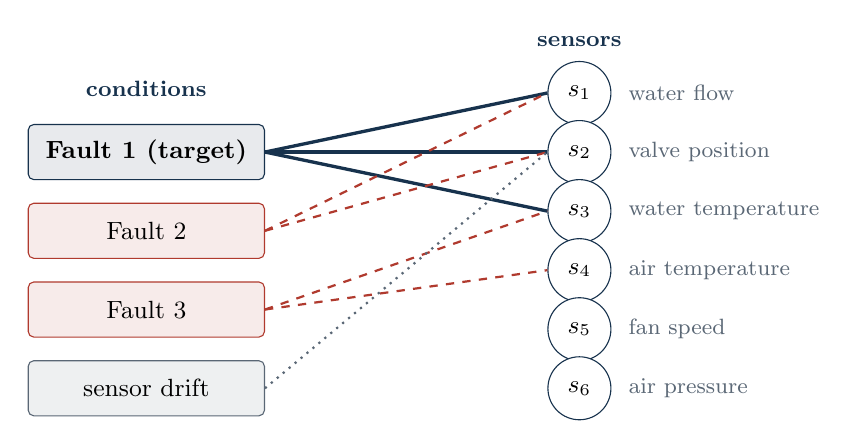
\begin{tikzpicture}[x=1mm,y=1mm,
    faultbase/.style={rounded corners=2pt,minimum width=30mm,minimum height=7mm,align=center,font=\small},
    faultN/.style={faultbase,draw=Navy,fill=Navy!10},
    faultR/.style={faultbase,draw=Red,fill=Red!10},
    faultM/.style={faultbase,draw=Muted,fill=Muted!10},
    sensor/.style={circle,draw=Navy,fill=white,minimum size=8mm,inner sep=0pt,font=\small},
    lbl/.style={font=\footnotesize,color=Muted,anchor=west}]
  % faults
  \node[faultN,font=\small\bfseries] (f1) at (0,30) {Fault 1 (target)};
  \node[faultR] (f2) at (0,20) {Fault 2};
  \node[faultR] (f3) at (0,10) {Fault 3};
  \node[faultM] (f4) at (0,0) {sensor drift};
  % sensors
  \foreach \i/\y/\name in {1/37.5/water flow,2/30/valve position,3/22.5/water temperature,4/15/air temperature,5/7.5/fan speed,6/0/air pressure}{
    \node[sensor] (s\i) at (55,\y) {$s_{\i}$};
    \node[lbl] at (60,\y) {\name};
  }
  % edges
  \foreach \s in {1,2,3}{\draw[Navy,very thick] (f1.east) -- (s\s.west);}
  \foreach \s in {1,2}{\draw[Red,thick,dashed] (f2.east) -- (s\s.west);}
  \foreach \s in {3,4}{\draw[Red,thick,dashed] (f3.east) -- (s\s.west);}
  \draw[Muted,thick,dotted] (f4.east) -- (s2.west);
  \node[font=\footnotesize\bfseries,color=Navy] at (0,38) {conditions};
  \node[font=\footnotesize\bfseries,color=Navy] at (55,44) {sensors};
\end{tikzpicture}
}
  \end{center}
  \end{column}
  \begin{column}{0.47\textwidth}
  \vspace{4mm}
  \begin{itemize}\setlength{\itemsep}{2.5mm}
    \item Every fault moves a \textbf{set} of sensors together: its \textbf{signature}.
    \item Signatures \textbf{overlap}: other faults and sensor errors move \emph{part} of Fault 1's signature.
    \item In practice we have labelled data for only \textbf{a few} faults. The others are unknown when the detector is built.
  \end{itemize}
  \end{column}
  \end{columns}
  \vspace{3mm}
  \takeaway{Goal: alarm on Fault 1, and stay quiet on everything else.}
  \note{0:45. A piece of equipment, for example a cooling unit in a building, has many sensors: water flow, valve position, temperatures, fan speed. A fault does not move one sensor; it moves a set of them together, its signature. Here Fault 1 moves s1, s2 and s3. Signatures overlap: Fault 2 moves two of the same sensors, Fault 3 moves one of them, and a drifting sensor moves one. In practice we only have labelled data for a few faults. A learned detector, for example a transformer with one token per sensor, is trained on normal windows and Fault 1 windows only. The goal is to alarm on Fault 1 and stay quiet on everything else.}
\end{frame}

% 3. Look-alike scenarios (unchanged)
\begin{frame}[t]{Look-alikes overlap with Fault 1 in many ways}
  \notation{illustration with reduced noise \(\cdot\) a window: a stretch of sensor readings over time \(\cdot\) shaded: the change after the onset}
  \vspace{1mm}
  \begin{center}
  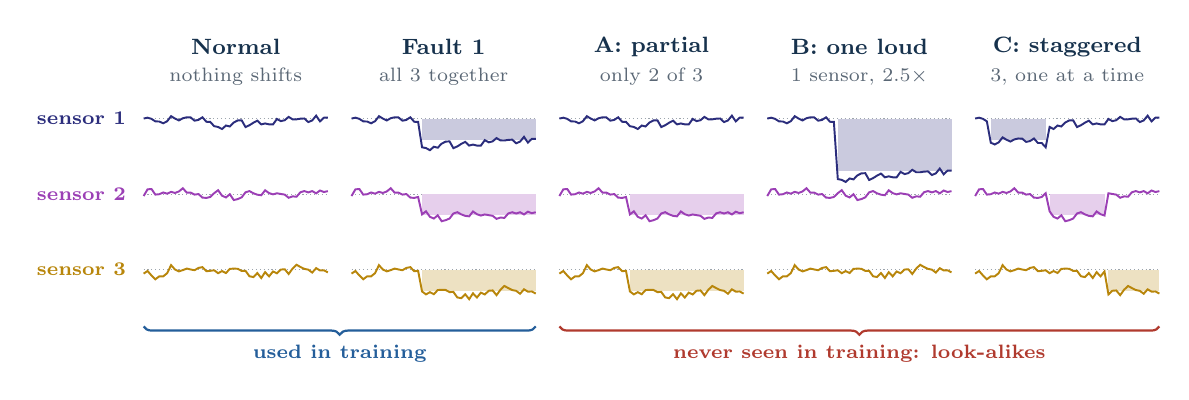
\begin{tikzpicture}
\node[font=\footnotesize\bfseries,color=Navy] at (11.70mm,9.12mm) {Normal};
\node[font=\scriptsize,color=Muted] at (11.70mm,5.28mm) {nothing shifts};
\draw[Muted!60,densely dotted] (0.00mm,0.00mm)--(23.40mm,0.00mm);
\draw[SensA,line width=0.7pt] (0.00mm,0.00mm) -- (0.50mm,0.11mm) -- (1.00mm,-0.04mm) -- (1.49mm,-0.36mm) -- (1.99mm,-0.38mm) -- (2.49mm,-0.60mm) -- (2.99mm,-0.34mm) -- (3.49mm,0.30mm) -- (3.98mm,-0.00mm) -- (4.48mm,-0.24mm) -- (4.98mm,0.04mm) -- (5.48mm,0.16mm) -- (5.97mm,0.14mm) -- (6.47mm,-0.27mm) -- (6.97mm,-0.17mm) -- (7.47mm,0.16mm) -- (7.97mm,-0.41mm) -- (8.46mm,-0.42mm) -- (8.96mm,-0.97mm) -- (9.46mm,-1.07mm) -- (9.96mm,-1.33mm) -- (10.46mm,-0.89mm) -- (10.95mm,-1.01mm) -- (11.45mm,-0.50mm) -- (11.95mm,-0.24mm) -- (12.45mm,-0.22mm) -- (12.94mm,-1.08mm) -- (13.44mm,-0.85mm) -- (13.94mm,-0.53mm) -- (14.44mm,-0.27mm) -- (14.94mm,-0.74mm) -- (15.43mm,-0.62mm) -- (15.93mm,-0.74mm) -- (16.43mm,-0.75mm) -- (16.93mm,-0.05mm) -- (17.43mm,-0.33mm) -- (17.92mm,-0.21mm) -- (18.42mm,0.21mm) -- (18.92mm,-0.10mm) -- (19.42mm,-0.10mm) -- (19.91mm,-0.02mm) -- (20.41mm,0.01mm) -- (20.91mm,-0.45mm) -- (21.41mm,-0.24mm) -- (21.91mm,0.37mm) -- (22.40mm,-0.36mm) -- (22.90mm,0.11mm) -- (23.40mm,0.11mm);
\draw[Muted!60,densely dotted] (0.00mm,-9.60mm)--(23.40mm,-9.60mm);
\draw[SensB,line width=0.7pt] (0.00mm,-9.84mm) -- (0.50mm,-8.99mm) -- (1.00mm,-8.95mm) -- (1.49mm,-9.66mm) -- (1.99mm,-9.61mm) -- (2.49mm,-9.39mm) -- (2.99mm,-9.54mm) -- (3.49mm,-9.31mm) -- (3.98mm,-9.45mm) -- (4.48mm,-9.26mm) -- (4.98mm,-8.85mm) -- (5.48mm,-9.41mm) -- (5.97mm,-9.41mm) -- (6.47mm,-9.66mm) -- (6.97mm,-9.59mm) -- (7.47mm,-10.04mm) -- (7.97mm,-10.08mm) -- (8.46mm,-9.96mm) -- (8.96mm,-9.48mm) -- (9.46mm,-9.10mm) -- (9.96mm,-9.80mm) -- (10.46mm,-10.02mm) -- (10.95mm,-9.61mm) -- (11.45mm,-10.35mm) -- (11.95mm,-10.23mm) -- (12.45mm,-10.01mm) -- (12.94mm,-9.37mm) -- (13.44mm,-9.21mm) -- (13.94mm,-9.49mm) -- (14.44mm,-9.67mm) -- (14.94mm,-9.74mm) -- (15.43mm,-9.11mm) -- (15.93mm,-9.47mm) -- (16.43mm,-9.63mm) -- (16.93mm,-9.49mm) -- (17.43mm,-9.58mm) -- (17.92mm,-9.66mm) -- (18.42mm,-10.06mm) -- (18.92mm,-9.88mm) -- (19.42mm,-9.93mm) -- (19.91mm,-9.36mm) -- (20.41mm,-9.21mm) -- (20.91mm,-9.38mm) -- (21.41mm,-9.21mm) -- (21.91mm,-9.50mm) -- (22.40mm,-9.14mm) -- (22.90mm,-9.33mm) -- (23.40mm,-9.22mm);
\draw[Muted!60,densely dotted] (0.00mm,-19.20mm)--(23.40mm,-19.20mm);
\draw[SensC,line width=0.7pt] (0.00mm,-19.69mm) -- (0.50mm,-19.36mm) -- (1.00mm,-19.93mm) -- (1.49mm,-20.41mm) -- (1.99mm,-20.04mm) -- (2.49mm,-20.04mm) -- (2.99mm,-19.64mm) -- (3.49mm,-18.62mm) -- (3.98mm,-19.17mm) -- (4.48mm,-19.41mm) -- (4.98mm,-19.25mm) -- (5.48mm,-19.05mm) -- (5.97mm,-19.17mm) -- (6.47mm,-19.26mm) -- (6.97mm,-18.97mm) -- (7.47mm,-18.87mm) -- (7.97mm,-19.39mm) -- (8.46mm,-19.34mm) -- (8.96mm,-19.27mm) -- (9.46mm,-19.64mm) -- (9.96mm,-19.37mm) -- (10.46mm,-19.62mm) -- (10.95mm,-19.09mm) -- (11.45mm,-19.06mm) -- (11.95mm,-19.08mm) -- (12.45mm,-19.35mm) -- (12.94mm,-19.34mm) -- (13.44mm,-20.03mm) -- (13.94mm,-20.13mm) -- (14.44mm,-19.62mm) -- (14.94mm,-20.25mm) -- (15.43mm,-19.51mm) -- (15.93mm,-20.04mm) -- (16.43mm,-19.42mm) -- (16.93mm,-19.65mm) -- (17.43mm,-19.18mm) -- (17.92mm,-19.14mm) -- (18.42mm,-19.74mm) -- (18.92mm,-19.05mm) -- (19.42mm,-18.57mm) -- (19.91mm,-18.85mm) -- (20.41mm,-19.09mm) -- (20.91mm,-19.19mm) -- (21.41mm,-19.56mm) -- (21.91mm,-19.00mm) -- (22.40mm,-19.29mm) -- (22.90mm,-19.27mm) -- (23.40mm,-19.54mm);
\node[font=\footnotesize\bfseries,color=Navy] at (38.10mm,9.12mm) {Fault 1};
\node[font=\scriptsize,color=Muted] at (38.10mm,5.28mm) {all 3 together};
\draw[Muted!60,densely dotted] (26.40mm,0.00mm)--(49.80mm,0.00mm);
\fill[SensA!25] (35.36mm,0.00mm) rectangle (49.80mm,-2.69mm);
\draw[SensA,line width=0.7pt] (26.40mm,0.00mm) -- (26.90mm,0.11mm) -- (27.40mm,-0.04mm) -- (27.89mm,-0.36mm) -- (28.39mm,-0.38mm) -- (28.89mm,-0.60mm) -- (29.39mm,-0.34mm) -- (29.89mm,0.30mm) -- (30.38mm,-0.00mm) -- (30.88mm,-0.24mm) -- (31.38mm,0.04mm) -- (31.88mm,0.16mm) -- (32.37mm,0.14mm) -- (32.87mm,-0.27mm) -- (33.37mm,-0.17mm) -- (33.87mm,0.16mm) -- (34.37mm,-0.41mm) -- (34.86mm,-0.42mm) -- (35.36mm,-3.65mm) -- (35.86mm,-3.75mm) -- (36.36mm,-4.02mm) -- (36.86mm,-3.58mm) -- (37.35mm,-3.70mm) -- (37.85mm,-3.19mm) -- (38.35mm,-2.93mm) -- (38.85mm,-2.90mm) -- (39.34mm,-3.76mm) -- (39.84mm,-3.54mm) -- (40.34mm,-3.22mm) -- (40.84mm,-2.96mm) -- (41.34mm,-3.43mm) -- (41.83mm,-3.31mm) -- (42.33mm,-3.43mm) -- (42.83mm,-3.44mm) -- (43.33mm,-2.74mm) -- (43.83mm,-3.02mm) -- (44.32mm,-2.90mm) -- (44.82mm,-2.48mm) -- (45.32mm,-2.78mm) -- (45.82mm,-2.79mm) -- (46.31mm,-2.71mm) -- (46.81mm,-2.68mm) -- (47.31mm,-3.14mm) -- (47.81mm,-2.93mm) -- (48.31mm,-2.32mm) -- (48.80mm,-3.05mm) -- (49.30mm,-2.58mm) -- (49.80mm,-2.58mm);
\draw[Muted!60,densely dotted] (26.40mm,-9.60mm)--(49.80mm,-9.60mm);
\fill[SensB!25] (35.36mm,-9.60mm) rectangle (49.80mm,-12.29mm);
\draw[SensB,line width=0.7pt] (26.40mm,-9.84mm) -- (26.90mm,-8.99mm) -- (27.40mm,-8.95mm) -- (27.89mm,-9.66mm) -- (28.39mm,-9.61mm) -- (28.89mm,-9.39mm) -- (29.39mm,-9.54mm) -- (29.89mm,-9.31mm) -- (30.38mm,-9.45mm) -- (30.88mm,-9.26mm) -- (31.38mm,-8.85mm) -- (31.88mm,-9.41mm) -- (32.37mm,-9.41mm) -- (32.87mm,-9.66mm) -- (33.37mm,-9.59mm) -- (33.87mm,-10.04mm) -- (34.37mm,-10.08mm) -- (34.86mm,-9.96mm) -- (35.36mm,-12.17mm) -- (35.86mm,-11.78mm) -- (36.36mm,-12.48mm) -- (36.86mm,-12.70mm) -- (37.35mm,-12.29mm) -- (37.85mm,-13.04mm) -- (38.35mm,-12.91mm) -- (38.85mm,-12.70mm) -- (39.34mm,-12.06mm) -- (39.84mm,-11.89mm) -- (40.34mm,-12.17mm) -- (40.84mm,-12.36mm) -- (41.34mm,-12.42mm) -- (41.83mm,-11.80mm) -- (42.33mm,-12.15mm) -- (42.83mm,-12.32mm) -- (43.33mm,-12.18mm) -- (43.83mm,-12.27mm) -- (44.32mm,-12.35mm) -- (44.82mm,-12.74mm) -- (45.32mm,-12.57mm) -- (45.82mm,-12.62mm) -- (46.31mm,-12.05mm) -- (46.81mm,-11.90mm) -- (47.31mm,-12.06mm) -- (47.81mm,-11.90mm) -- (48.31mm,-12.18mm) -- (48.80mm,-11.83mm) -- (49.30mm,-12.02mm) -- (49.80mm,-11.90mm);
\draw[Muted!60,densely dotted] (26.40mm,-19.20mm)--(49.80mm,-19.20mm);
\fill[SensC!25] (35.36mm,-19.20mm) rectangle (49.80mm,-21.89mm);
\draw[SensC,line width=0.7pt] (26.40mm,-19.69mm) -- (26.90mm,-19.36mm) -- (27.40mm,-19.93mm) -- (27.89mm,-20.41mm) -- (28.39mm,-20.04mm) -- (28.89mm,-20.04mm) -- (29.39mm,-19.64mm) -- (29.89mm,-18.62mm) -- (30.38mm,-19.17mm) -- (30.88mm,-19.41mm) -- (31.38mm,-19.25mm) -- (31.88mm,-19.05mm) -- (32.37mm,-19.17mm) -- (32.87mm,-19.26mm) -- (33.37mm,-18.97mm) -- (33.87mm,-18.87mm) -- (34.37mm,-19.39mm) -- (34.86mm,-19.34mm) -- (35.36mm,-21.96mm) -- (35.86mm,-22.33mm) -- (36.36mm,-22.05mm) -- (36.86mm,-22.31mm) -- (37.35mm,-21.78mm) -- (37.85mm,-21.75mm) -- (38.35mm,-21.77mm) -- (38.85mm,-22.04mm) -- (39.34mm,-22.02mm) -- (39.84mm,-22.72mm) -- (40.34mm,-22.81mm) -- (40.84mm,-22.31mm) -- (41.34mm,-22.94mm) -- (41.83mm,-22.20mm) -- (42.33mm,-22.73mm) -- (42.83mm,-22.11mm) -- (43.33mm,-22.34mm) -- (43.83mm,-21.87mm) -- (44.32mm,-21.83mm) -- (44.82mm,-22.43mm) -- (45.32mm,-21.74mm) -- (45.82mm,-21.26mm) -- (46.31mm,-21.53mm) -- (46.81mm,-21.78mm) -- (47.31mm,-21.88mm) -- (47.81mm,-22.25mm) -- (48.31mm,-21.69mm) -- (48.80mm,-21.98mm) -- (49.30mm,-21.96mm) -- (49.80mm,-22.23mm);
\node[font=\footnotesize\bfseries,color=Navy] at (64.50mm,9.12mm) {A: partial};
\node[font=\scriptsize,color=Muted] at (64.50mm,5.28mm) {only 2 of 3};
\draw[Muted!60,densely dotted] (52.80mm,0.00mm)--(76.20mm,0.00mm);
\draw[SensA,line width=0.7pt] (52.80mm,0.00mm) -- (53.30mm,0.11mm) -- (53.80mm,-0.04mm) -- (54.29mm,-0.36mm) -- (54.79mm,-0.38mm) -- (55.29mm,-0.60mm) -- (55.79mm,-0.34mm) -- (56.29mm,0.30mm) -- (56.78mm,-0.00mm) -- (57.28mm,-0.24mm) -- (57.78mm,0.04mm) -- (58.28mm,0.16mm) -- (58.77mm,0.14mm) -- (59.27mm,-0.27mm) -- (59.77mm,-0.17mm) -- (60.27mm,0.16mm) -- (60.77mm,-0.41mm) -- (61.26mm,-0.42mm) -- (61.76mm,-0.97mm) -- (62.26mm,-1.07mm) -- (62.76mm,-1.33mm) -- (63.26mm,-0.89mm) -- (63.75mm,-1.01mm) -- (64.25mm,-0.50mm) -- (64.75mm,-0.24mm) -- (65.25mm,-0.22mm) -- (65.74mm,-1.08mm) -- (66.24mm,-0.85mm) -- (66.74mm,-0.53mm) -- (67.24mm,-0.27mm) -- (67.74mm,-0.74mm) -- (68.23mm,-0.62mm) -- (68.73mm,-0.74mm) -- (69.23mm,-0.75mm) -- (69.73mm,-0.05mm) -- (70.23mm,-0.33mm) -- (70.72mm,-0.21mm) -- (71.22mm,0.21mm) -- (71.72mm,-0.10mm) -- (72.22mm,-0.10mm) -- (72.71mm,-0.02mm) -- (73.21mm,0.01mm) -- (73.71mm,-0.45mm) -- (74.21mm,-0.24mm) -- (74.71mm,0.37mm) -- (75.20mm,-0.36mm) -- (75.70mm,0.11mm) -- (76.20mm,0.11mm);
\draw[Muted!60,densely dotted] (52.80mm,-9.60mm)--(76.20mm,-9.60mm);
\fill[SensB!25] (61.76mm,-9.60mm) rectangle (76.20mm,-12.29mm);
\draw[SensB,line width=0.7pt] (52.80mm,-9.84mm) -- (53.30mm,-8.99mm) -- (53.80mm,-8.95mm) -- (54.29mm,-9.66mm) -- (54.79mm,-9.61mm) -- (55.29mm,-9.39mm) -- (55.79mm,-9.54mm) -- (56.29mm,-9.31mm) -- (56.78mm,-9.45mm) -- (57.28mm,-9.26mm) -- (57.78mm,-8.85mm) -- (58.28mm,-9.41mm) -- (58.77mm,-9.41mm) -- (59.27mm,-9.66mm) -- (59.77mm,-9.59mm) -- (60.27mm,-10.04mm) -- (60.77mm,-10.08mm) -- (61.26mm,-9.96mm) -- (61.76mm,-12.17mm) -- (62.26mm,-11.78mm) -- (62.76mm,-12.48mm) -- (63.26mm,-12.70mm) -- (63.75mm,-12.29mm) -- (64.25mm,-13.04mm) -- (64.75mm,-12.91mm) -- (65.25mm,-12.70mm) -- (65.74mm,-12.06mm) -- (66.24mm,-11.89mm) -- (66.74mm,-12.17mm) -- (67.24mm,-12.36mm) -- (67.74mm,-12.42mm) -- (68.23mm,-11.80mm) -- (68.73mm,-12.15mm) -- (69.23mm,-12.32mm) -- (69.73mm,-12.18mm) -- (70.23mm,-12.27mm) -- (70.72mm,-12.35mm) -- (71.22mm,-12.74mm) -- (71.72mm,-12.57mm) -- (72.22mm,-12.62mm) -- (72.71mm,-12.05mm) -- (73.21mm,-11.90mm) -- (73.71mm,-12.06mm) -- (74.21mm,-11.90mm) -- (74.71mm,-12.18mm) -- (75.20mm,-11.83mm) -- (75.70mm,-12.02mm) -- (76.20mm,-11.90mm);
\draw[Muted!60,densely dotted] (52.80mm,-19.20mm)--(76.20mm,-19.20mm);
\fill[SensC!25] (61.76mm,-19.20mm) rectangle (76.20mm,-21.89mm);
\draw[SensC,line width=0.7pt] (52.80mm,-19.69mm) -- (53.30mm,-19.36mm) -- (53.80mm,-19.93mm) -- (54.29mm,-20.41mm) -- (54.79mm,-20.04mm) -- (55.29mm,-20.04mm) -- (55.79mm,-19.64mm) -- (56.29mm,-18.62mm) -- (56.78mm,-19.17mm) -- (57.28mm,-19.41mm) -- (57.78mm,-19.25mm) -- (58.28mm,-19.05mm) -- (58.77mm,-19.17mm) -- (59.27mm,-19.26mm) -- (59.77mm,-18.97mm) -- (60.27mm,-18.87mm) -- (60.77mm,-19.39mm) -- (61.26mm,-19.34mm) -- (61.76mm,-21.96mm) -- (62.26mm,-22.33mm) -- (62.76mm,-22.05mm) -- (63.26mm,-22.31mm) -- (63.75mm,-21.78mm) -- (64.25mm,-21.75mm) -- (64.75mm,-21.77mm) -- (65.25mm,-22.04mm) -- (65.74mm,-22.02mm) -- (66.24mm,-22.72mm) -- (66.74mm,-22.81mm) -- (67.24mm,-22.31mm) -- (67.74mm,-22.94mm) -- (68.23mm,-22.20mm) -- (68.73mm,-22.73mm) -- (69.23mm,-22.11mm) -- (69.73mm,-22.34mm) -- (70.23mm,-21.87mm) -- (70.72mm,-21.83mm) -- (71.22mm,-22.43mm) -- (71.72mm,-21.74mm) -- (72.22mm,-21.26mm) -- (72.71mm,-21.53mm) -- (73.21mm,-21.78mm) -- (73.71mm,-21.88mm) -- (74.21mm,-22.25mm) -- (74.71mm,-21.69mm) -- (75.20mm,-21.98mm) -- (75.70mm,-21.96mm) -- (76.20mm,-22.23mm);
\node[font=\footnotesize\bfseries,color=Navy] at (90.90mm,9.12mm) {B: one loud};
\node[font=\scriptsize,color=Muted] at (90.90mm,5.28mm) {1 sensor, 2.5$\times$};
\draw[Muted!60,densely dotted] (79.20mm,0.00mm)--(102.60mm,0.00mm);
\fill[SensA!25] (88.16mm,0.00mm) rectangle (102.60mm,-6.72mm);
\draw[SensA,line width=0.7pt] (79.20mm,0.00mm) -- (79.70mm,0.11mm) -- (80.20mm,-0.04mm) -- (80.69mm,-0.36mm) -- (81.19mm,-0.38mm) -- (81.69mm,-0.60mm) -- (82.19mm,-0.34mm) -- (82.69mm,0.30mm) -- (83.18mm,-0.00mm) -- (83.68mm,-0.24mm) -- (84.18mm,0.04mm) -- (84.68mm,0.16mm) -- (85.17mm,0.14mm) -- (85.67mm,-0.27mm) -- (86.17mm,-0.17mm) -- (86.67mm,0.16mm) -- (87.17mm,-0.41mm) -- (87.66mm,-0.42mm) -- (88.16mm,-7.69mm) -- (88.66mm,-7.79mm) -- (89.16mm,-8.05mm) -- (89.66mm,-7.61mm) -- (90.15mm,-7.73mm) -- (90.65mm,-7.22mm) -- (91.15mm,-6.96mm) -- (91.65mm,-6.94mm) -- (92.14mm,-7.80mm) -- (92.64mm,-7.57mm) -- (93.14mm,-7.25mm) -- (93.64mm,-6.99mm) -- (94.14mm,-7.46mm) -- (94.63mm,-7.34mm) -- (95.13mm,-7.46mm) -- (95.63mm,-7.47mm) -- (96.13mm,-6.77mm) -- (96.63mm,-7.05mm) -- (97.12mm,-6.93mm) -- (97.62mm,-6.51mm) -- (98.12mm,-6.82mm) -- (98.62mm,-6.82mm) -- (99.11mm,-6.74mm) -- (99.61mm,-6.71mm) -- (100.11mm,-7.17mm) -- (100.61mm,-6.96mm) -- (101.11mm,-6.35mm) -- (101.60mm,-7.08mm) -- (102.10mm,-6.61mm) -- (102.60mm,-6.61mm);
\draw[Muted!60,densely dotted] (79.20mm,-9.60mm)--(102.60mm,-9.60mm);
\draw[SensB,line width=0.7pt] (79.20mm,-9.84mm) -- (79.70mm,-8.99mm) -- (80.20mm,-8.95mm) -- (80.69mm,-9.66mm) -- (81.19mm,-9.61mm) -- (81.69mm,-9.39mm) -- (82.19mm,-9.54mm) -- (82.69mm,-9.31mm) -- (83.18mm,-9.45mm) -- (83.68mm,-9.26mm) -- (84.18mm,-8.85mm) -- (84.68mm,-9.41mm) -- (85.17mm,-9.41mm) -- (85.67mm,-9.66mm) -- (86.17mm,-9.59mm) -- (86.67mm,-10.04mm) -- (87.17mm,-10.08mm) -- (87.66mm,-9.96mm) -- (88.16mm,-9.48mm) -- (88.66mm,-9.10mm) -- (89.16mm,-9.80mm) -- (89.66mm,-10.02mm) -- (90.15mm,-9.61mm) -- (90.65mm,-10.35mm) -- (91.15mm,-10.23mm) -- (91.65mm,-10.01mm) -- (92.14mm,-9.37mm) -- (92.64mm,-9.21mm) -- (93.14mm,-9.49mm) -- (93.64mm,-9.67mm) -- (94.14mm,-9.74mm) -- (94.63mm,-9.11mm) -- (95.13mm,-9.47mm) -- (95.63mm,-9.63mm) -- (96.13mm,-9.49mm) -- (96.63mm,-9.58mm) -- (97.12mm,-9.66mm) -- (97.62mm,-10.06mm) -- (98.12mm,-9.88mm) -- (98.62mm,-9.93mm) -- (99.11mm,-9.36mm) -- (99.61mm,-9.21mm) -- (100.11mm,-9.38mm) -- (100.61mm,-9.21mm) -- (101.11mm,-9.50mm) -- (101.60mm,-9.14mm) -- (102.10mm,-9.33mm) -- (102.60mm,-9.22mm);
\draw[Muted!60,densely dotted] (79.20mm,-19.20mm)--(102.60mm,-19.20mm);
\draw[SensC,line width=0.7pt] (79.20mm,-19.69mm) -- (79.70mm,-19.36mm) -- (80.20mm,-19.93mm) -- (80.69mm,-20.41mm) -- (81.19mm,-20.04mm) -- (81.69mm,-20.04mm) -- (82.19mm,-19.64mm) -- (82.69mm,-18.62mm) -- (83.18mm,-19.17mm) -- (83.68mm,-19.41mm) -- (84.18mm,-19.25mm) -- (84.68mm,-19.05mm) -- (85.17mm,-19.17mm) -- (85.67mm,-19.26mm) -- (86.17mm,-18.97mm) -- (86.67mm,-18.87mm) -- (87.17mm,-19.39mm) -- (87.66mm,-19.34mm) -- (88.16mm,-19.27mm) -- (88.66mm,-19.64mm) -- (89.16mm,-19.37mm) -- (89.66mm,-19.62mm) -- (90.15mm,-19.09mm) -- (90.65mm,-19.06mm) -- (91.15mm,-19.08mm) -- (91.65mm,-19.35mm) -- (92.14mm,-19.34mm) -- (92.64mm,-20.03mm) -- (93.14mm,-20.13mm) -- (93.64mm,-19.62mm) -- (94.14mm,-20.25mm) -- (94.63mm,-19.51mm) -- (95.13mm,-20.04mm) -- (95.63mm,-19.42mm) -- (96.13mm,-19.65mm) -- (96.63mm,-19.18mm) -- (97.12mm,-19.14mm) -- (97.62mm,-19.74mm) -- (98.12mm,-19.05mm) -- (98.62mm,-18.57mm) -- (99.11mm,-18.85mm) -- (99.61mm,-19.09mm) -- (100.11mm,-19.19mm) -- (100.61mm,-19.56mm) -- (101.11mm,-19.00mm) -- (101.60mm,-19.29mm) -- (102.10mm,-19.27mm) -- (102.60mm,-19.54mm);
\node[font=\footnotesize\bfseries,color=Navy] at (117.30mm,9.12mm) {C: staggered};
\node[font=\scriptsize,color=Muted] at (117.30mm,5.28mm) {3, one at a time};
\draw[Muted!60,densely dotted] (105.60mm,0.00mm)--(129.00mm,0.00mm);
\fill[SensA!25] (107.59mm,0.00mm) rectangle (114.56mm,-2.69mm);
\draw[SensA,line width=0.7pt] (105.60mm,0.00mm) -- (106.10mm,0.11mm) -- (106.60mm,-0.04mm) -- (107.09mm,-0.36mm) -- (107.59mm,-3.07mm) -- (108.09mm,-3.29mm) -- (108.59mm,-3.03mm) -- (109.09mm,-2.39mm) -- (109.58mm,-2.69mm) -- (110.08mm,-2.92mm) -- (110.58mm,-2.65mm) -- (111.08mm,-2.53mm) -- (111.57mm,-2.55mm) -- (112.07mm,-2.96mm) -- (112.57mm,-2.86mm) -- (113.07mm,-2.53mm) -- (113.57mm,-3.10mm) -- (114.06mm,-3.11mm) -- (114.56mm,-3.65mm) -- (115.06mm,-1.07mm) -- (115.56mm,-1.33mm) -- (116.06mm,-0.89mm) -- (116.55mm,-1.01mm) -- (117.05mm,-0.50mm) -- (117.55mm,-0.24mm) -- (118.05mm,-0.22mm) -- (118.54mm,-1.08mm) -- (119.04mm,-0.85mm) -- (119.54mm,-0.53mm) -- (120.04mm,-0.27mm) -- (120.54mm,-0.74mm) -- (121.03mm,-0.62mm) -- (121.53mm,-0.74mm) -- (122.03mm,-0.75mm) -- (122.53mm,-0.05mm) -- (123.03mm,-0.33mm) -- (123.52mm,-0.21mm) -- (124.02mm,0.21mm) -- (124.52mm,-0.10mm) -- (125.02mm,-0.10mm) -- (125.51mm,-0.02mm) -- (126.01mm,0.01mm) -- (126.51mm,-0.45mm) -- (127.01mm,-0.24mm) -- (127.51mm,0.37mm) -- (128.00mm,-0.36mm) -- (128.50mm,0.11mm) -- (129.00mm,0.11mm);
\draw[Muted!60,densely dotted] (105.60mm,-9.60mm)--(129.00mm,-9.60mm);
\fill[SensB!25] (115.06mm,-9.60mm) rectangle (122.03mm,-12.29mm);
\draw[SensB,line width=0.7pt] (105.60mm,-9.84mm) -- (106.10mm,-8.99mm) -- (106.60mm,-8.95mm) -- (107.09mm,-9.66mm) -- (107.59mm,-9.61mm) -- (108.09mm,-9.39mm) -- (108.59mm,-9.54mm) -- (109.09mm,-9.31mm) -- (109.58mm,-9.45mm) -- (110.08mm,-9.26mm) -- (110.58mm,-8.85mm) -- (111.08mm,-9.41mm) -- (111.57mm,-9.41mm) -- (112.07mm,-9.66mm) -- (112.57mm,-9.59mm) -- (113.07mm,-10.04mm) -- (113.57mm,-10.08mm) -- (114.06mm,-9.96mm) -- (114.56mm,-9.48mm) -- (115.06mm,-11.78mm) -- (115.56mm,-12.48mm) -- (116.06mm,-12.70mm) -- (116.55mm,-12.29mm) -- (117.05mm,-13.04mm) -- (117.55mm,-12.91mm) -- (118.05mm,-12.70mm) -- (118.54mm,-12.06mm) -- (119.04mm,-11.89mm) -- (119.54mm,-12.17mm) -- (120.04mm,-12.36mm) -- (120.54mm,-12.42mm) -- (121.03mm,-11.80mm) -- (121.53mm,-12.15mm) -- (122.03mm,-12.32mm) -- (122.53mm,-9.49mm) -- (123.03mm,-9.58mm) -- (123.52mm,-9.66mm) -- (124.02mm,-10.06mm) -- (124.52mm,-9.88mm) -- (125.02mm,-9.93mm) -- (125.51mm,-9.36mm) -- (126.01mm,-9.21mm) -- (126.51mm,-9.38mm) -- (127.01mm,-9.21mm) -- (127.51mm,-9.50mm) -- (128.00mm,-9.14mm) -- (128.50mm,-9.33mm) -- (129.00mm,-9.22mm);
\draw[Muted!60,densely dotted] (105.60mm,-19.20mm)--(129.00mm,-19.20mm);
\fill[SensC!25] (122.53mm,-19.20mm) rectangle (129.00mm,-21.89mm);
\draw[SensC,line width=0.7pt] (105.60mm,-19.69mm) -- (106.10mm,-19.36mm) -- (106.60mm,-19.93mm) -- (107.09mm,-20.41mm) -- (107.59mm,-20.04mm) -- (108.09mm,-20.04mm) -- (108.59mm,-19.64mm) -- (109.09mm,-18.62mm) -- (109.58mm,-19.17mm) -- (110.08mm,-19.41mm) -- (110.58mm,-19.25mm) -- (111.08mm,-19.05mm) -- (111.57mm,-19.17mm) -- (112.07mm,-19.26mm) -- (112.57mm,-18.97mm) -- (113.07mm,-18.87mm) -- (113.57mm,-19.39mm) -- (114.06mm,-19.34mm) -- (114.56mm,-19.27mm) -- (115.06mm,-19.64mm) -- (115.56mm,-19.37mm) -- (116.06mm,-19.62mm) -- (116.55mm,-19.09mm) -- (117.05mm,-19.06mm) -- (117.55mm,-19.08mm) -- (118.05mm,-19.35mm) -- (118.54mm,-19.34mm) -- (119.04mm,-20.03mm) -- (119.54mm,-20.13mm) -- (120.04mm,-19.62mm) -- (120.54mm,-20.25mm) -- (121.03mm,-19.51mm) -- (121.53mm,-20.04mm) -- (122.03mm,-19.42mm) -- (122.53mm,-22.34mm) -- (123.03mm,-21.87mm) -- (123.52mm,-21.83mm) -- (124.02mm,-22.43mm) -- (124.52mm,-21.74mm) -- (125.02mm,-21.26mm) -- (125.51mm,-21.53mm) -- (126.01mm,-21.78mm) -- (126.51mm,-21.88mm) -- (127.01mm,-22.25mm) -- (127.51mm,-21.69mm) -- (128.00mm,-21.98mm) -- (128.50mm,-21.96mm) -- (129.00mm,-22.23mm);
\node[anchor=east,font=\scriptsize\bfseries,color=SensA] at (-1mm,0.00mm) {sensor 1};
\node[anchor=east,font=\scriptsize\bfseries,color=SensB] at (-1mm,-9.60mm) {sensor 2};
\node[anchor=east,font=\scriptsize\bfseries,color=SensC] at (-1mm,-19.20mm) {sensor 3};
\draw[Blue,thick,decorate,decoration={brace,mirror,amplitude=3pt}] (0mm,-26.40mm) -- (49.80mm,-26.40mm) node[midway,below=3pt,font=\scriptsize\bfseries,color=Blue] {used in training};
\draw[Red,thick,decorate,decoration={brace,mirror,amplitude=3pt}] (52.80mm,-26.40mm) -- (129.00mm,-26.40mm) node[midway,below=3pt,font=\scriptsize\bfseries,color=Red] {never seen in training: look-alikes};
\end{tikzpicture}

  \end{center}
  \vspace{1mm}
  \takeaway{The training data contain only the two left panels. The detector never learns why A, B and C are not Fault 1.}
  \note{0:45. These are the kinds of look-alikes. Fault 1: all three sensors drop together. A: only two of the three move. B: one sensor moves a lot. C: all three move, but at different times. None of them is Fault 1. On the LBNL fan-coil data, a transformer trained on normal versus Fault 1 catches every Fault 1 window, but also alarms on 99 percent of two-of-three windows. The training data contain only normal and Fault 1, so nothing tells the detector that A, B or C are different. The question is which rule it learns.}
\end{frame}

% 4. Setup: evidence, SUM and AND, example table
\begin{frame}[t]{Setup: the evidence of each sensor, and two ways to combine it}
  \notation{\(a_j\): evidence of sensor \(j\) \(\cdot\) \(S\): the sensors Fault 1 moves (its signature), \(k=|S|\) \(\cdot\) example: Fault 1 moves each of its 3 sensors by 3 noise units}
  \lead{\textbf{Evidence of sensor \(j\)}: how far it moved after the onset, in units of its noise.}
  \vspace{-1mm}
  \[
    \bx{a_j=\frac{\text{mean before onset}-\text{mean after onset}}{\text{noise level of sensor }j}}
  \]
  \vspace{-1mm}
  \begin{columns}[T,onlytextwidth]
  \begin{column}{0.44\textwidth}
  \begin{lemblock}{SUM: combine all evidence}
    \vspace{-2mm}
    \[ f_{\mathrm{SUM}}(a)=\sum_{j\in S}a_j \]
    \vspace{-4mm}
  \end{lemblock}
  \vspace{0.5mm}
  \begin{lemblock}{AND: require every sensor}
    \vspace{-2mm}
    \[ f_{\mathrm{AND}}(a)=\min_{j\in S}a_j \]
    \vspace{-4mm}
  \end{lemblock}
  \end{column}
  \begin{column}{0.53\textwidth}
  \vspace{1mm}
  \begin{center}
  {\fontsize{9}{11}\selectfont\renewcommand{\arraystretch}{1.32}\setlength{\tabcolsep}{2.6mm}
  \begin{tabular}{@{}llcc@{}}
    \toprule
    & \textbf{Evidence} & \textbf{SUM} & \textbf{Minimum}\\
    \midrule
    {\color{Muted}Fault 1} & \((3,3,3)\) & 9 & 3\\
    {\color{Muted}2 of 3 move} & \((3,3,0)\) & 6 & \textcolor{Red}{\textbf{0}}\\
    {\color{Muted}1 of 3 moves} & \((3,0,0)\) & 3 & \textcolor{Red}{\textbf{0}}\\
    \bottomrule
  \end{tabular}\par}
  \end{center}
  \end{column}
  \end{columns}
  \keybox{Key distinction.}{SUM asks whether the \textbf{total} evidence is high. AND asks whether the \textbf{weakest} required sensor also provides sufficient evidence.}
  \note{1:00. To analyse this we summarise each sensor by one number, its evidence a\_j: how far the sensor moved after the onset, in units of its own noise. There are two natural ways to combine these numbers. The SUM adds the evidence of the fault's sensors; the AND takes the minimum, so it asks whether every sensor moved. In the table Fault 1 moves each of its three sensors by 3. Both rules identify the complete fault: the SUM is 9 and the minimum is 3. But if only two sensors move, the SUM is still 6 while the minimum is 0, and with one sensor the SUM is 3 and the minimum is still 0. Both rules identify the complete fault, but only the minimum-based rule directly penalizes a missing sensor.}
\end{frame}

% 5. Mathematical problem setting + training versus deployment
\begin{frame}[t]{Mathematical setting: training versus deployment}
  \notation{\(a\): sensor-evidence vector \(\cdot\) \(\sigma\): noise standard deviation \(\cdot\) \(\delta\): fault-induced shift \(\cdot\) \(S\): signature sensors, \(k=|S|\) \(\cdot\) \(C\): total number of sensor tokens \(\cdot\) \(\mathbf 1_S\): 1 on the sensors of \(S\) \(\cdot\) \(e_j\): unit vector of sensor \(j\)}
  \begin{columns}[T,onlytextwidth]
  \begin{column}{0.47\textwidth}
  \begin{lemblock}{Gaussian evidence model}
    \vspace{-3mm}
    \[
      \begin{aligned}
        \text{Normal: }&a\sim\mathcal N(0,\sigma^2 I)\\
        \text{Fault 1: }&a\sim\mathcal N(\delta\mathbf 1_S,\sigma^2 I)\\
        \text{Look-alike: }&a\sim\mathcal N(\mu,\sigma^2 I),\quad \operatorname{supp}(\mu)\subsetneq S
      \end{aligned}
    \]
    A look-alike shifts only a \textbf{proper subset} of Fault 1's sensors.\\[0.8mm]
    \textbf{Near-miss}: misses exactly one sensor, \(\mu=\delta(\mathbf 1_S-e_j)\), e.g.\ \((3,3,0)\).
  \end{lemblock}
  \end{column}
  \begin{column}{0.5\textwidth}
  \begin{lemblock}{Training problem: a simple hypothesis test}
    \vspace{-2mm}
    \[ H_0:\text{Normal}\quad\text{vs}\quad H_1:\text{Fault 1} \]
    \vspace{-4mm}
  \end{lemblock}
  \vspace{1mm}
  \begin{thmblock}{Deployment problem: a composite hypothesis test}
    \vspace{-2mm}
    \[ H_1:\text{Fault 1}\quad\text{vs}\quad H_0:\text{Normal}\ +\ \text{all look-alikes} \]
    \vspace{-4mm}
  \end{thmblock}
  \end{column}
  \end{columns}
  \keybox{Main insight.}{A rule that is optimal for the training test need not be valid for the deployment test.}
  \note{1:10. We use a Gaussian evidence model to isolate the effect of the aggregation rule. Normal windows have mean zero; Fault 1 shifts each of its k sensors by delta; a look-alike shifts only a proper subset of the sensors associated with the target fault. The look-alike that misses exactly one sensor is called a near-miss, for example (3,3,0); it will matter later. The real difference is between two statistical problems. Training asks a simple test: normal or Fault 1. Deployment asks a composite test: Fault 1, or normal or any look-alike. A rule that is optimal for the training test need not be valid for the deployment test. This mismatch between the two statistical problems motivates the first two theorems.}
\end{frame}

% ---------------- Theorem 1(i) ----------------
\begin{frame}[t]{Theorem 1(i): the SUM is optimal for training}
  \notation{\(p_0,p_1\): density of the evidence under Normal and under Fault 1 \(\cdot\) \(\Lambda\): likelihood ratio}
  \begin{qblock}{Question}
    What is the most powerful detector for Normal versus one complete fault?
  \end{qblock}
  \vspace{1mm}
  \lead{The Neyman--Pearson lemma says: threshold the likelihood ratio}
  \vspace{-2.5mm}
  \[ \Lambda(a)=\frac{p_1(a)}{p_0(a)} \]
  \vspace{-1.5mm}
  \lead{Under independent, equal-variance Gaussian evidence:}
  \vspace{-2.5mm}
  \[ \log\Lambda(a)=\frac{\delta}{\sigma^2}\sum_{j\in S}a_j-\frac{k\delta^2}{2\sigma^2} \]
  \vspace{-1.5mm}
  \lead{Therefore:\qquad \bx{\text{Optimal rule: threshold the SUM}}}
  \proofidea{Independence turns density products into sums after taking logarithms; the equal-variance Gaussian likelihood ratio is linear in the evidence.}
  \note{1:00. The first question: what is the most powerful detector for normal versus one complete fault? The Neyman--Pearson lemma says to threshold the likelihood ratio. Under independent, equal-variance Gaussian evidence, the log likelihood ratio is a constant times the sum of the evidence of the fault's sensors, minus a constant. So the optimal rule thresholds the SUM. SUM is not just a convenient baseline. It is the statistically optimal rule for the two training distributions under these assumptions.}
\end{frame}

% ---------------- Theorem 1(ii) ----------------
\begin{frame}[t]{Theorem 1(ii): how often are look-alikes flagged?}
  \notation{\(\alpha\): false-alarm rate on Normal \(\cdot\) \(\beta_{\rm det}\): detection rate on Fault 1 \(\cdot\) \(z_\alpha=\Phi^{-1}(1-\alpha)\), 2.33 for \(\alpha=1\%\) \(\cdot\) \(\Phi\): standard normal CDF \(\cdot\) \(h\): mean evidence of the look-alike}
  \lead{For a linear detector \(w^\top a\), define}
  \vspace{-2.5mm}
  \[ r_h=\frac{w^\top h}{w^\top(\delta\mathbf 1_S)} \]
  \vspace{-1.5mm}
  \lead{This is the \textbf{fraction of Fault 1's signal} reproduced by the look-alike. The paper derives:}
  \vspace{1mm}
  \begin{thmblock}{Theorem 1(ii)}
    \vspace{-2mm}
    \[ P(\text{alarm}\mid h)=\Phi\Big(r_h\big[\Phi^{-1}(\beta_{\rm det})+z_\alpha\big]-z_\alpha\Big) \]
    \vspace{-4mm}
  \end{thmblock}
  \vspace{1mm}
  \lead{For the SUM and a look-alike shifting \(m\) of \(k\) sensors:\qquad \(r_h=\dfrac{m}{k}\).}
  \takeaway{The better the detector catches Fault 1, the more look-alikes it flags.}
  \note{1:00. Theorem 1 also says how often look-alikes are flagged. For a linear detector w-transpose-a, r\_h is the fraction of the target-fault signal that the look-alike reproduces. The alarm probability on that look-alike is this closed-form expression, where alpha is the normal false-alarm rate and beta\_det is the target-fault detection rate. For the SUM and a look-alike that shifts m of the k sensors, r\_h is m over k. The theorem gives a direct relationship between how much of the fault signal a look-alike reproduces and how likely the detector is to flag it: the better the detector catches Fault 1, the more look-alikes it flags.}
\end{frame}

% ---------------- Theorem 1(ii) numbers ----------------
\begin{frame}[t]{Theorem 1(ii): numerical implication}
  \notation{example from the report: SUM detector, \(k=3\) sensors, \(\delta/\sigma=3\), \(\alpha=1\%\) false alarms on Normal}
  \lead{Consider}
  \vspace{-2.5mm}
  \[ k=3,\qquad \alpha=0.01,\qquad \beta_{\rm det}=0.998,\qquad r_h=\tfrac23 . \]
  \vspace{-1.5mm}
  \lead{The theorem predicts}
  \vspace{-2.5mm}
  \[ P(\text{alarm}\mid\text{two-of-three})\approx0.87 . \]
  \vspace{1mm}
  \begin{center}
  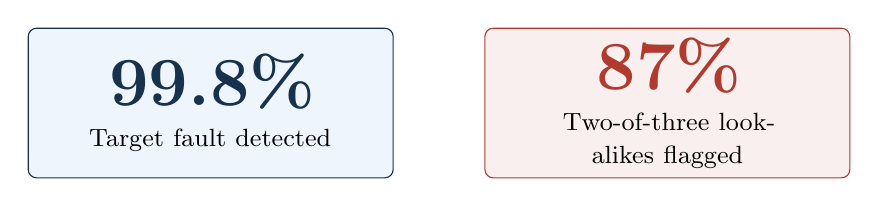
\begin{tikzpicture}
    \node[draw=Navy,fill=LightBlue!40,rounded corners=3pt,text width=44mm,align=center,minimum height=19mm] (a) at (0,0)
      {{\fontsize{24}{28}\selectfont\bfseries\color{Navy}99.8\%}\\[1mm]{\fontsize{9.5}{11}\selectfont Target fault detected}};
    \node[draw=Red,fill=Red!8,rounded corners=3pt,text width=44mm,align=center,minimum height=19mm] (b) at (58mm,0)
      {{\fontsize{24}{28}\selectfont\bfseries\color{Red}87\%}\\[1mm]{\fontsize{9.5}{11}\selectfont Two-of-three look-alikes flagged}};
  \end{tikzpicture}
  \end{center}
  \proofidea{Calibrate the Gaussian score threshold using \(\alpha\), infer its target mean from \(\beta_{\rm det}\), and scale that mean by \(r_h\) for the look-alike.}
  \note{0:40. A concrete case: three sensors, one percent false alarms, and a detector that catches 99.8 percent of Fault 1. A two-of-three look-alike reproduces two thirds of the signal, and the theorem predicts that it is flagged 87 percent of the time. The detector is excellent on its intended task, but it flags most partial signatures. The proof: calibrate the Gaussian score threshold with alpha, infer the target mean from the detection rate, and scale that mean by r\_h for the look-alike. This is the failure that the next theorem addresses.}
\end{frame}

% ---------------- Theorem 2: validity ----------------
\begin{frame}[t]{Theorem 2: what makes a detector valid?}
  \notation{\(P_0\): probability under Normal \(\cdot\) \(P_\mu\): probability under a look-alike with mean \(\mu\) \(\cdot\) \(z_\alpha\): threshold for false-alarm rate \(\alpha\) (2.33 for 1\%)}
  \begin{columns}[T,onlytextwidth]
  \begin{column}{0.46\textwidth}
  \lead{A \textbf{valid} detector must satisfy}
  \vspace{-1mm}
  \[ \begin{aligned} &P_0(\text{alarm})\le\alpha\\ \text{and}\quad &P_\mu(\text{alarm})\le\alpha\quad\text{for every look-alike }\mu . \end{aligned} \]
  \vspace{1mm}
  \lead{The AND detector:}
  \vspace{1mm}
  \begin{center}
  \bx{\text{Alarm only if }\ \min_{j\in S}\frac{a_j}{\sigma}>z_\alpha}
  \end{center}
  \end{column}
  \begin{column}{0.5\textwidth}
  \textbf{Why is it valid?}
  \vspace{1mm}

  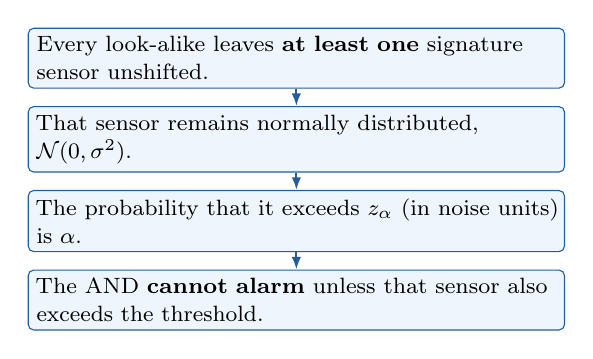
\begin{tikzpicture}[node distance=2.2mm]
    \node[stepbox=66mm] (s1) {Every look-alike leaves \textbf{at least one} signature sensor unshifted.};
    \node[stepbox=66mm,below=of s1] (s2) {That sensor remains normally distributed, \(\mathcal N(0,\sigma^2)\).};
    \node[stepbox=66mm,below=of s2] (s3) {The probability that it exceeds \(z_\alpha\) (in noise units) is \(\alpha\).};
    \node[stepbox=66mm,below=of s3] (s4) {The AND \textbf{cannot alarm} unless that sensor also exceeds the threshold.};
    \draw[farrow] (s1)--(s2); \draw[farrow] (s2)--(s3); \draw[farrow] (s3)--(s4);
  \end{tikzpicture}
  \end{column}
  \end{columns}
  \takeaway{So the AND alarms with probability at most \(\alpha\) under every look-alike: it is valid.}
  \note{1:00. A valid detector must raise at most alpha alarms on normal windows and on every look-alike. The AND detector alarms only if the smallest standardized evidence exceeds z\_alpha. Why is it valid? Every look-alike leaves at least one signature sensor unshifted. That sensor remains normally distributed. The probability that it exceeds z\_alpha is alpha. And the AND cannot alarm unless that sensor also exceeds the threshold. One missing sensor is enough to protect the AND detector. Even if every other shifted sensor becomes extremely large, the unshifted sensor controls the false-alarm probability.}
\end{frame}

% ---------------- Theorem 2: limits of additive detectors ----------------
\begin{frame}[t]{Theorem 2: limits of additive detectors}
  \notation{\(M\): strength of a look-alike on each shifted sensor \(\cdot\) \(\delta\): Fault 1's shift per sensor \(\cdot\) \(\beta_{\rm det}\): detection rate on Fault 1 \(\cdot\) \(\alpha\): false-alarm rate}
  \lead{What happens when look-alikes become \textbf{stronger}? For a look-alike shifting \(k-1\) sensors with strength \(M\), the total evidence grows with \((k-1)M\).}
  \vspace{1.5mm}
  \begin{thmblock}{Theorem 2(c): sums break down}
    For the best valid non-negative linear detector,
    \[ M\ge\frac{k}{k-1}\,\delta\quad\Longrightarrow\quad\beta_{\rm det}\le\alpha . \]
    For \(k=3\): look-alikes \(1.5\times\) as strong as Fault 1 are enough.
  \end{thmblock}
  \vspace{1mm}
  \textbf{It also shows:}
  {\fontsize{8.7}{10.5}\selectfont
  \begin{itemize}\setlength{\itemsep}{0.4mm}
    \item[\textcolor{Green}{\(\checkmark\)}] The AND is valid for \textbf{every} look-alike strength.
    \item[\textcolor{Green}{\(\checkmark\)}] When \(M\ge\delta\), the AND misses Fault 1 at most \(k\) times as often as the best valid detector.
    \item[\textcolor{Red}{\(\times\)}] For unbounded look-alike strength, no finite-threshold additive detector with a nondecreasing, unbounded term is valid.
  \end{itemize}\par}
  \takeaway{A structural limit of adding evidence. Next: can a transformer compute an AND instead?}
  \note{0:50. What happens when look-alikes become stronger? A look-alike that shifts k minus 1 sensors with strength M has total evidence k minus 1 times M. Once M reaches k over k minus 1 times delta, its total equals Fault 1's, and the best valid non-negative linear detector is useless; for three sensors, 1.5 times as strong is enough. The theorem also shows the AND is valid for every strength and misses at most k times as often as the best valid detector, and that with unbounded look-alikes no additive detector is valid. So the detector must be able to compute an AND. Can a transformer?}
\end{frame}

% ---------------- Bridge: where attention comes in ----------------
\begin{frame}[t]{Where attention comes in: from sensor tokens to one score}
  \notation{token: the representation of one sensor \(\cdot\) query, key: learned vectors that score each token \(\cdot\) \(\pi_j\): attention weight of sensor \(j\) \(\cdot\) \(u,c\): weight and bias of the output head}
  \lead{A transformer detector turns each sensor into a \textbf{token}. In its last step, \textbf{attention pooling} combines the tokens into one score:}
  \vspace{2mm}
  \begin{center}
  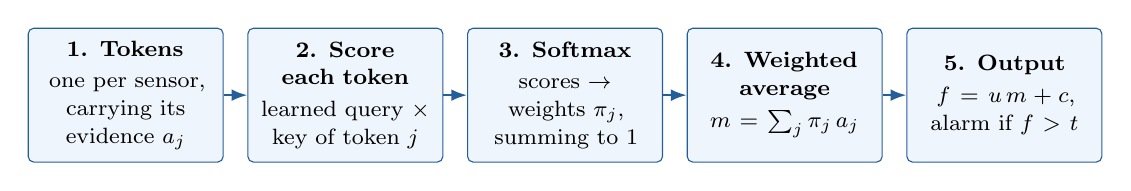
\begin{tikzpicture}[node distance=3mm,
      st/.style={draw=Blue,fill=LightBlue!40,rounded corners=2pt,align=center,inner sep=2.5pt,text width=23mm,minimum height=17mm,font=\fontsize{8.3}{10}\selectfont},
      ar/.style={-{Latex[length=2mm]},Blue,thick}]
    \node[st] (t) {\textbf{1. Tokens}\\[0.5mm] one per sensor,\\ carrying its evidence \(a_j\)};
    \node[st,right=of t] (s) {\textbf{2. Score each token}\\[0.5mm] learned query \(\times\) key of token \(j\)};
    \node[st,right=of s] (w) {\textbf{3. Softmax}\\[0.5mm] scores \(\to\) weights \(\pi_j\),\\ summing to 1};
    \node[st,right=of w] (m) {\textbf{4. Weighted average}\\[0.5mm] \(m=\sum_j\pi_j\,a_j\)};
    \node[st,right=of m] (f) {\textbf{5. Output}\\[0.5mm] \(f=u\,m+c\),\\ alarm if \(f>t\)};
    \draw[ar] (t)--(s); \draw[ar] (s)--(w); \draw[ar] (w)--(m); \draw[ar] (m)--(f);
  \end{tikzpicture}
  \end{center}
  \vspace{2mm}
  \lead{Each token carries one evidence number, so the score of token \(j\) is \(q_a\,a_j+b_j\). The analysis keeps the evidence part and writes \(\beta=-q_a\):\qquad \bx{\text{score of token } j=-\beta\,a_j}}
  \vspace{1.5mm}
  {\body At equal attention, training moves only this coefficient of the full pooling layer (Remark 1 in the report), so one number is enough to study.\par}
  \takeaway{One learned number, \(\beta\), decides how the pooled score combines the sensors.}
  \note{0:50. Theorem 2 says a safe detector must be able to compute an AND. How does a transformer combine sensors? Each sensor becomes a token. In the last step, attention pooling scores each token with a learned query and key, the softmax turns the scores into weights that sum to one, the weights average the evidence, and a linear head gives the final score. In our setting each token carries one evidence number, so the score of token j is q\_a times a\_j plus a bias. The analysis keeps the evidence part and calls minus q\_a beta. Why is one number enough? At equal attention, the gradient of the full pooling layer points only along this coefficient. So beta decides how the pooled score combines the sensors.}
\end{frame}

% ---------------- Attention ----------------
\begin{frame}[t]{Softmax attention: one parameter between OR, SUM and AND}
  \notation{\(\pi_j\): attention weight of sensor \(j\) \(\cdot\) \(\beta\): inverse temperature of the softmax \(\cdot\) \(u,c\): weight and bias of the output head \(\cdot\) example: near-miss \((3,3,0)\)}
  \lead{With token scores \(-\beta a_j\), the softmax gives the attention average:}
  \vspace{-1mm}
  \[ m_\beta(a)=\sum_j\pi_j\,a_j,\qquad \pi_j=\frac{e^{-\beta a_j}}{\sum_\ell e^{-\beta a_\ell}} \]
  \lead{The \textbf{inverse temperature} \(\beta\) controls the aggregation:}
  \vspace{1mm}
  \begin{center}
  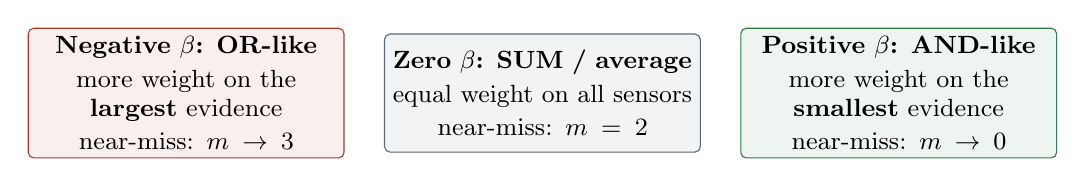
\begin{tikzpicture}[node distance=5mm]
    \node[regime=Red] (or) {\textbf{Negative \(\beta\): OR-like}\\[0.6mm] more weight on the \textbf{largest} evidence\\[0.6mm] near-miss: \(m\to3\)};
    \node[regime=Muted,right=of or] (sum) {\textbf{Zero \(\beta\): SUM / average}\\[0.6mm] equal weight on all sensors\\[0.6mm] near-miss: \(m=2\)};
    \node[regime=Green,right=of sum] (and) {\textbf{Positive \(\beta\): AND-like}\\[0.6mm] more weight on the \textbf{smallest} evidence\\[0.6mm] near-miss: \(m\to0\)};
  \end{tikzpicture}
  \end{center}
  \vspace{0.5mm}
  \lead{The complete score is \quad \(f_\theta(a)=u\,m_\beta(a)+c\), \quad \(\theta=(\beta,u,c)\).}
  \takeaway{Which \(\beta\) does training choose? That needs the gradient \(\partial L/\partial\beta\), which rests on two facts (next slide).}
  \note{0:45. With token scores minus beta a\_j, the softmax gives this attention average. The inverse temperature beta controls the aggregation. Negative beta puts more weight on the largest evidence: OR-like; on the near-miss (3,3,0) the average goes to 3. Zero beta gives equal weights, the average 2: the SUM. Positive beta puts more weight on the smallest evidence: AND-like, and the near-miss average goes to 0. So the inverse temperature provides a trainable path between OR, SUM and AND. The question is which beta training chooses. To answer it we need the gradient of the loss with respect to beta, and that rests on two facts, on the next slide.}
\end{frame}

% ---------------- Lemmas ----------------
\begin{frame}[t]{Two mathematical observations}
  \notation{\(\bar a\): mean evidence across sensors \(\cdot\) \(S^2(a)\): spread of the evidence across sensors \(\cdot\) \(\operatorname{Var}_{\pi_\beta}\): variance under the attention weights \(\cdot\) \(\ell\): logistic loss \(\cdot\) \(y=\pm1\): label}
  \begin{qblock}{Why we need them}
    Theorem 3 needs the \textbf{sign} of \(\partial L/\partial\beta=\mathbb E\big[\ell'(yf)\,y\,u\,\partial_\beta m_\beta(a)\big]\) (chain rule): how \(\beta\) changes the pooled score (Lemma 2), and how large that change is in each class (Lemma 1).
  \end{qblock}
  \vspace{1mm}
  \begin{columns}[T,onlytextwidth]
  \begin{column}{0.485\textwidth}
  \begin{lemblock}{Lemma 1: sensor spread}
    \[ \begin{aligned} S^2(a)&=\tfrac1C\textstyle\sum_j(a_j-\bar a)^2\\[0.5mm] \mathbb E\big[S^2(a)\mid\bar a\big]&=s_0+\Delta(\mu) \end{aligned} \]
    \(s_0\): noise part, the \textbf{same for every class}.\\
    \(\Delta(\mu)\): spread of the class mean. \(\Delta=0\) for Normal and (if \(C=k\)) Fault 1; \(\Delta>0\) for a near-miss.
  \end{lemblock}
  \end{column}
  \begin{column}{0.485\textwidth}
  \begin{lemblock}{Lemma 2: attention derivative}
    \[ \bx{\frac{\partial m_\beta(a)}{\partial\beta}=-\operatorname{Var}_{\pi_\beta}(a)} \]
    At equal attention (\(\beta=0\)): \ \(\partial_\beta m_\beta=-S^2(a)\).\\[0.8mm]
    The more uneven the evidence, the faster raising \(\beta\) lowers the score.
  \end{lemblock}
  \end{column}
  \end{columns}
  \proofidea{Lemma 2: differentiate the softmax weights. Lemma 1: \(\bar a\) is independent of the deviations \(a_j-\bar a\).}
  \note{0:50. Why do we need these two facts? Theorem 3 asks for the sign of the gradient of the loss in beta, and by the chain rule that needs the derivative of the pooled score in beta. Lemma 2 gives it: minus the variance of the evidence under the attention weights, and at equal attention minus the spread. So the more uneven a window, the faster raising beta lowers its score. Lemma 1 says how large the spread is in each class: a noise part, the same for every class, plus the spread of the class mean, which is zero for normal and Fault 1 windows and positive for a near-miss.}
\end{frame}

% ---------------- Theorem 3 (statement) ----------------
\begin{frame}[t]{Theorem 3: which way does training move \(\beta\)?}
  \notation{\(\pi_t,\pi_{\rm nm}\): shares of Fault 1 and near-miss windows \(\cdot\) \(\Delta_t,\Delta_{\rm nm}\): spread of the Fault 1 and near-miss means \(\cdot\) \(\operatorname{sig}\): sigmoid \(\cdot\) \(u^\star\!>0\), \(f\): weight and score of the best SUM rule}
  \begin{qblock}{Question}
    Start at the SUM (\(\beta=0\)). Does training push \(\beta\) \textbf{up}, toward the AND, or \textbf{down}, toward an OR?
  \end{qblock}
  \vspace{1mm}
  \lead{The paper derives the gradient in closed form:}
  \vspace{-1mm}
  \[
    \left.\frac{\partial L}{\partial\beta}\right|_{\rm SUM}
    =u^\star\Big[\,{\color{Red}\pi_t\,\Delta_t\,\mathbb E_t[\operatorname{sig}(-f)]}
    \;-\;{\color{Green}\pi_{\rm nm}\,\Delta_{\rm nm}\,\mathbb E_{\rm nm}[\operatorname{sig}(f)]}\,\Big]
  \]
  \vspace{-1mm}
  {\fontsize{8.8}{10.8}\selectfont \textcolor{Red}{\textbf{Fault 1 windows}} push \(\beta\) down (if uneven).\qquad \textcolor{Green}{\textbf{Near-misses}} push \(\beta\) up.\par}
  \vspace{1.5mm}
  \begin{thmblock}{Result (only Fault 1's sensors, \(C=k\))}
    Fault 1 windows are even on average (\(\Delta_t=0\)); near-misses are not (\(\Delta_{\rm nm}>0\)). So \(\partial L/\partial\beta<0\): gradient descent \textbf{increases} \(\beta\), toward the AND.
  \end{thmblock}
  \proofidea{Chain rule and Lemma 2; Lemma 1 splits the spread; the noise part cancels because the SUM rule's intercept is optimal.}
  \note{1:00. Theorem 3. Start at the SUM, equal attention, and ask which way training pushes beta. The paper derives the gradient in closed form. It has two terms. Each is a share of a class, times the spread of that class's mean, times how wrong the SUM rule is on that class. Fault 1 windows, if they are uneven, push beta down; near-misses push beta up. When the only tokens are Fault 1's sensors, Fault 1 windows are even on average, so their term vanishes, and the near-miss term is positive. So the gradient is negative and gradient descent increases beta: attention moves toward the AND. The proof uses the chain rule and Lemma 2, splits the spread with Lemma 1, and the common noise term cancels because the intercept of the SUM rule is optimal. The near-miss creates the spread that drives the gradient. This is the core mathematical reason attention moves from SUM towards AND.}
\end{frame}

% ---------------- Theorem 3 (what it means) ----------------
\begin{frame}[t]{Theorem 3: what the training data do to \(\beta\)}
  \notation{\(C\): number of sensor tokens \(\cdot\) \(k\): number of Fault 1's sensors (\(C>k\): extra sensors that Fault 1 does not move) \(\cdot\) head refit: the output weight and bias are fitted at each step}
  \vspace{1mm}
  \begin{center}
  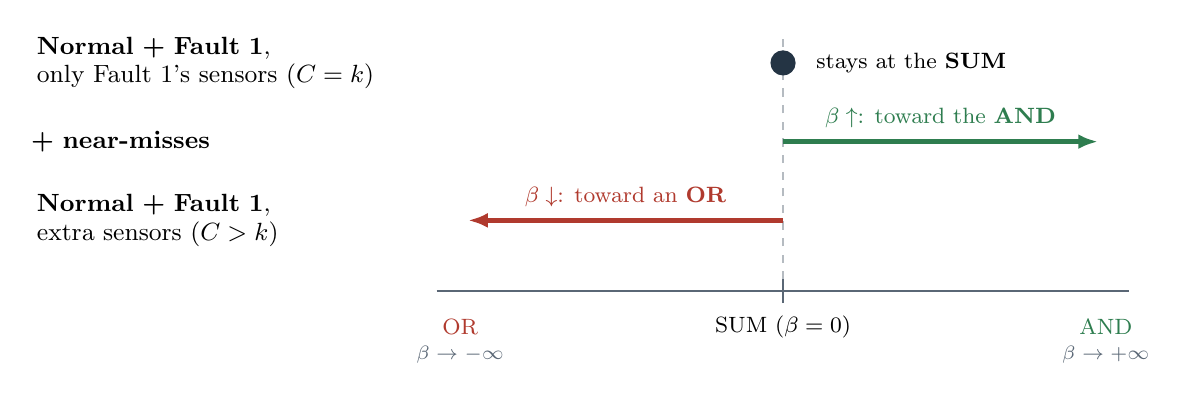
\begin{tikzpicture}[x=1mm,y=1mm]
    % axis
    \draw[Muted,thick] (52,0) -- (140,0);
    \draw[Muted,thick] (96,-1.5) -- (96,1.5);
    \draw[Muted!45,dashed] (96,1.5) -- (96,33);
    \node[font=\footnotesize,Red] at (55,-4.5) {OR};
    \node[font=\footnotesize] at (96,-4.5) {SUM (\(\beta=0\))};
    \node[font=\footnotesize,Green] at (137,-4.5) {AND};
    \node[font=\scriptsize,Muted] at (55,-8) {\(\beta\to-\infty\)};
    \node[font=\scriptsize,Muted] at (137,-8) {\(\beta\to+\infty\)};
    % row a
    \node[anchor=west,text width=48mm,font=\fontsize{8.6}{10.3}\selectfont] at (0,29) {\textbf{Normal + Fault 1},\\ only Fault 1's sensors (\(C=k\))};
    \fill[Ink] (96,29) circle (1.6);
    \node[anchor=west,font=\fontsize{8.4}{10}\selectfont] at (99,29) {stays at the \textbf{SUM}};
    % row b
    \node[anchor=west,text width=48mm,font=\fontsize{8.6}{10.3}\selectfont] at (0,19) {\textbf{+ near-misses}};
    \draw[-{Latex[length=2.5mm]},Green,line width=1.6pt] (96,19) -- (136,19);
    \node[anchor=south,font=\fontsize{8.4}{10}\selectfont,Green] at (116,19.5) {\(\beta\uparrow\): toward the \textbf{AND}};
    % row c
    \node[anchor=west,text width=48mm,font=\fontsize{8.6}{10.3}\selectfont] at (0,9) {\textbf{Normal + Fault 1},\\ extra sensors (\(C>k\))};
    \draw[-{Latex[length=2.5mm]},Red,line width=1.6pt] (96,9) -- (56,9);
    \node[anchor=south,font=\fontsize{8.4}{10}\selectfont,Red] at (76,9.5) {\(\beta\downarrow\): toward an \textbf{OR}};
  \end{tikzpicture}
  \end{center}
  \vspace{1mm}
  \keybox{(d) Starting elsewhere.}{With near-misses, and the output head refit at each step, every start with \(\beta(0)\ge0\) ends at an AND, soft or hard: never back at the SUM, never at an OR.}
  \vspace{1.5mm}
  \takeaway{Near-misses move attention toward the AND. Next: how far does \(\beta\) go?}
  \note{0:45. What does this mean for the three kinds of training data? With only normal and Fault 1 windows and only Fault 1's sensors, attention stays at the SUM. Add near-misses and beta goes up, toward the AND. With extra sensors that Fault 1 does not move, beta goes down, toward an OR; we will see this in the experiments. Part (d) covers other starting points: with near-misses and the output head refit at each step, every start with beta at least zero ends at an AND, soft or hard, never back at the SUM or at an OR. The next question is how far beta goes.}
\end{frame}

% ---------------- Theorem 4 (why) ----------------
\begin{frame}[t]{Theorem 4: how far does \(\beta\) go?}
  \notation{hard AND: \(\beta\to\infty\), the score follows the single weakest sensor \(\cdot\) soft AND: a finite \(\beta^\star>0\) \(\cdot\) \(\delta\): Fault 1's shift per sensor}
  \begin{qblock}{Why we need Theorem 4}
    Theorem 3 gives only the \textbf{direction} at \(\beta=0\). Does \(\beta\) run off to \(+\infty\), the hard AND, or does it stop?
  \end{qblock}
  \vspace{1mm}
  \begin{columns}[T,onlytextwidth]
  \begin{column}{0.485\textwidth}
  \begin{lemblock}{Without noise}
    Fault 1 is exactly \((\delta,\delta,\delta)\), a near-miss exactly \((\delta,\delta,0)\).\\
    A larger \(\beta\) always lowers the near-miss score and never hurts Fault 1.
    \vspace{1mm}
    \begin{center}
    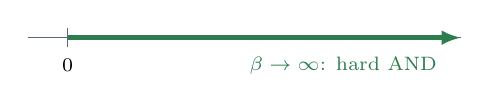
\begin{tikzpicture}[x=1mm,y=1mm]
      \draw[Muted] (0,0) -- (55,0); \draw[Muted] (5,-1.2) -- (5,1.2);
      \node[font=\scriptsize] at (5,-3.5) {\(0\)};
      \draw[-{Latex[length=2.5mm]},Green,line width=1.6pt] (5,0) -- (55,0);
      \node[font=\scriptsize,Green] at (40,-3.5) {\(\beta\to\infty\): hard AND};
    \end{tikzpicture}
    \end{center}
  \end{lemblock}
  \end{column}
  \begin{column}{0.485\textwidth}
  \begin{lemblock}{With noise}
    Real Fault 1 windows are \textbf{randomly uneven}. A very large \(\beta\) follows the weakest sensor and misses some of them.
    \vspace{1mm}
    \begin{center}
    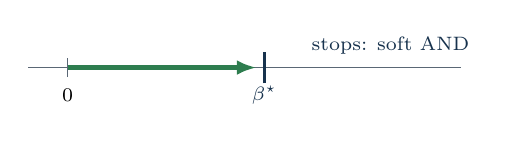
\begin{tikzpicture}[x=1mm,y=1mm]
      \draw[Muted] (0,0) -- (55,0); \draw[Muted] (5,-1.2) -- (5,1.2);
      \node[font=\scriptsize] at (5,-3.5) {\(0\)};
      \draw[-{Latex[length=2.5mm]},Green,line width=1.6pt] (5,0) -- (29,0);
      \draw[Navy,line width=1.2pt] (30,-2) -- (30,2);
      \node[font=\scriptsize,Navy] at (30,-3.5) {\(\beta^\star\)};
      \node[font=\scriptsize,Navy] at (46,2.8) {stops: soft AND};
    \end{tikzpicture}
    \end{center}
  \end{lemblock}
  \end{column}
  \end{columns}
  \takeaway{Near-misses push \(\beta\) up; uneven Fault 1 windows push back. Noise is what keeps the AND soft.}
  \note{0:45. Why do we need Theorem 4? Theorem 3 gives only the direction at beta equal to zero. Does beta run off to infinity, the hard AND, or does it stop? Without noise, Fault 1 is exactly delta on every sensor and a near-miss is exactly delta, delta, zero. A larger beta always lowers the near-miss score and never hurts Fault 1, so beta goes to infinity: the hard AND. With noise, real Fault 1 windows are randomly uneven. A very large beta makes the score follow the weakest sensor, and it starts missing some real faults. So near-misses push beta up and uneven Fault 1 windows push back. Noise is what keeps the AND soft.}
\end{frame}

% ---------------- Theorem 4 (result) ----------------
\begin{frame}[t]{Theorem 4: a soft AND that grows with the near-miss share}
  \notation{\(\rho\): share of near-misses in training \(\cdot\) \(\beta^\star(\rho)\): where training settles \(\cdot\) \(\kappa\): slope of \(\beta^\star\) in \(\rho\) \(\cdot\) plot: loss with the best head for each \(\beta\), two sensors, \(\delta/\sigma=2\) (report, Appendix D); dots: minima}
  \begin{columns}[T,onlytextwidth]
  \begin{column}{0.5\textwidth}
  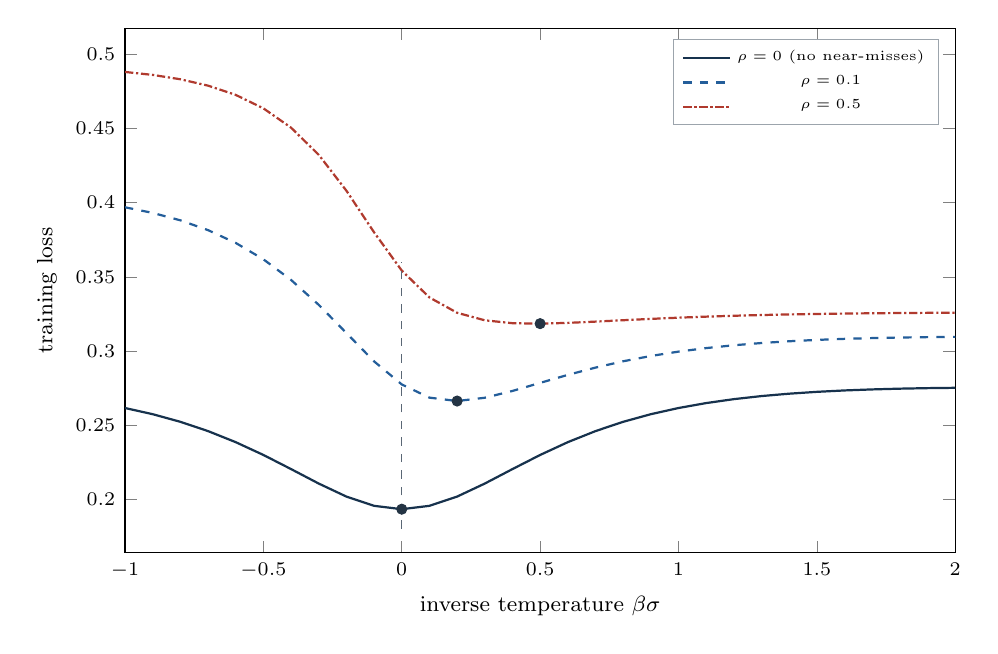
\begin{tikzpicture}
    \begin{axis}[width=\linewidth,height=0.68\linewidth,xmin=-1,xmax=2,
      xlabel={inverse temperature \(\beta\sigma\)},ylabel={training loss},
      tick label style={font=\scriptsize},
      legend style={font=\tiny,at={(0.98,0.98)},anchor=north east,draw=Muted!60}]
      \addplot[no marks,thick,color=Navy] coordinates {(-1.0,0.26139) (-0.9,0.25722) (-0.8,0.25207) (-0.7,0.24580) (-0.6,0.23833) (-0.5,0.22969) (-0.4,0.22015) (-0.3,0.21038) (-0.2,0.20158) (-0.1,0.19534) (-0.0,0.19307) (0.1,0.19534) (0.2,0.20158) (0.3,0.21038) (0.4,0.22015) (0.5,0.22969) (0.6,0.23833) (0.7,0.24580) (0.8,0.25207) (0.9,0.25722) (1.0,0.26139) (1.1,0.26473) (1.2,0.26738) (1.3,0.26946) (1.4,0.27107) (1.5,0.27231) (1.6,0.27326) (1.7,0.27395) (1.8,0.27446) (1.9,0.27481) (2.0,0.27503)};
\addlegendentry{$\rho=0$ (no near-misses)}
\addplot[no marks,thick,color=Blue,dashed] coordinates {(-1.0,0.39692) (-0.9,0.39314) (-0.8,0.38812) (-0.7,0.38151) (-0.6,0.37288) (-0.5,0.36180) (-0.4,0.34788) (-0.3,0.33106) (-0.2,0.31202) (-0.1,0.29289) (-0.0,0.27731) (0.1,0.26840) (0.2,0.26610) (0.3,0.26832) (0.4,0.27291) (0.5,0.27836) (0.6,0.28376) (0.7,0.28868) (0.8,0.29295) (0.9,0.29653) (1.0,0.29947) (1.1,0.30186) (1.2,0.30377) (1.3,0.30528) (1.4,0.30647) (1.5,0.30739) (1.6,0.30809) (1.7,0.30861) (1.8,0.30899) (1.9,0.30926) (2.0,0.30944)};
\addlegendentry{$\rho=0.1$}
\addplot[no marks,thick,color=Red,densely dashdotted] coordinates {(-1.0,0.48832) (-0.9,0.48632) (-0.8,0.48338) (-0.7,0.47907) (-0.6,0.47282) (-0.5,0.46375) (-0.4,0.45070) (-0.3,0.43236) (-0.2,0.40811) (-0.1,0.38003) (-0.0,0.35419) (0.1,0.33606) (0.2,0.32570) (0.3,0.32062) (0.4,0.31866) (0.5,0.31836) (0.6,0.31887) (0.7,0.31973) (0.8,0.32067) (0.9,0.32157) (1.0,0.32239) (1.1,0.32309) (1.2,0.32369) (1.3,0.32418) (1.4,0.32458) (1.5,0.32490) (1.6,0.32516) (1.7,0.32537) (1.8,0.32553) (1.9,0.32565) (2.0,0.32574)};
\addlegendentry{$\rho=0.5$}
\addplot[only marks,mark=*,mark size=1.8pt,color=Ink,forget plot] coordinates {(-0.0,0.19307) (0.2,0.26610) (0.5,0.31836)};

      \draw[Muted,dashed] (axis cs:0,0.18) -- (axis cs:0,0.36);
    \end{axis}
  \end{tikzpicture}
  \end{column}
  \begin{column}{0.47\textwidth}
  \begin{thmblock}{Theorem 4}
    (i) Training stops at a \textbf{finite} \(\beta^\star\):
    \[ \beta^\star(\rho)=\kappa\,\rho+O(\rho^2),\qquad\kappa>0. \]
    \(\kappa\) = how strongly the SUM rule mistakes near-misses for Fault 1, divided by the curvature of the loss.\\[1mm]
    (ii) For a small \(\rho\), every start in a fixed interval around \(\beta=0\) reaches \(\beta^\star\).
  \end{thmblock}
  \end{column}
  \end{columns}
  \proofidea{Follow the minimiser from the SUM as \(\rho\) grows (implicit function theorem); a Schur complement isolates \(\beta\).}
  \takeaway{More near-misses give sharper attention, but it stays finite: a soft AND.}
  \note{1:00. Here is the answer. The plot is the training loss as a function of beta, with the output head fitted for each beta, for two sensors. Without near-misses the minimum is at zero, the SUM. With 10 percent near-misses it moves to the right, and with 50 percent further right, but it stays finite. Theorem 4 makes this exact: training stops at a finite inverse temperature beta-star, which grows linearly in the near-miss share rho with slope kappa. Kappa is how strongly the SUM rule mistakes near-misses for Fault 1, divided by the curvature of the loss. Part (ii): for a small share, every start in a fixed interval around zero reaches this soft AND, including starts that lean slightly toward an OR. The proof follows the minimiser from the SUM as rho grows, using the implicit function theorem, and a Schur complement isolates beta. More near-misses give sharper attention, but it stays finite: a soft AND.}
\end{frame}

% ---------------- Experiments ----------------
\begin{frame}[t]{Experiments: objective and setup}
  \notation{window: \(C\) sensors \(\times\) 48 time steps \(\cdot\) \(\pi_j\): attention weight of sensor \(j\) \(\cdot\) 1\% false alarms on normal windows throughout \(\cdot\) 3 random seeds}
  \begin{qblock}{Objective}
    Do Theorems 1--4 hold for a transformer trained on \textbf{raw time series}?
    \textbf{Why it matters:} the theory uses one number per sensor and a reduced attention model.
  \end{qblock}
  \vspace{0.5mm}
  \begin{columns}[T,onlytextwidth]
  \begin{column}{0.485\textwidth}
  \begin{lemblock}{Synthetic series}
    20 sensors, 48 steps. Fault 1: 3 sensors drop by \(2.5\sigma\).
  \end{lemblock}
  \end{column}
  \begin{column}{0.485\textwidth}
  \begin{lemblock}{LBNL fan-coil unit (simulated building data)}
    24 sensors, 48 steps of 15 min. Fault 1: fan-outlet blockage.
  \end{lemblock}
  \end{column}
  \end{columns}
  \vspace{0.5mm}
  \begin{center}
  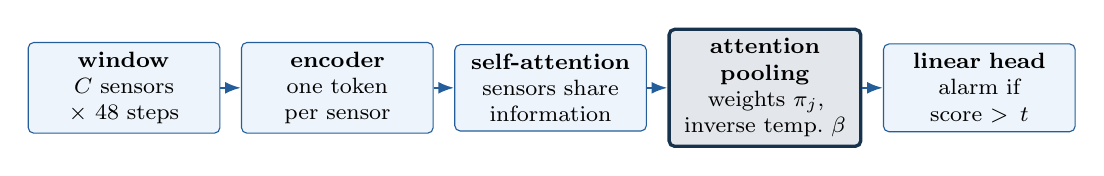
\begin{tikzpicture}[node distance=2.6mm,
      lay/.style={draw=Blue,fill=LightBlue!45,rounded corners=2pt,align=center,minimum height=9.5mm,text width=22mm,font=\fontsize{8}{9.5}\selectfont},
      hl/.style={draw=Navy,fill=Navy!12,very thick,rounded corners=2pt,align=center,minimum height=9.5mm,text width=22mm,font=\fontsize{8}{9.5}\selectfont},
      ar/.style={-{Latex[length=2mm]},Blue,thick}]
    \node[lay] (in) {\textbf{window}\\ \(C\) sensors \(\times\) 48 steps};
    \node[lay,right=of in] (enc) {\textbf{encoder}\\ one token per sensor};
    \node[lay,right=of enc] (sa) {\textbf{self-attention}\\ sensors share information};
    \node[hl,right=of sa] (pool) {\textbf{attention pooling}\\ weights \(\pi_j\), inverse temp.\ \(\beta\)};
    \node[lay,right=of pool] (out) {\textbf{linear head}\\ alarm if score \(>t\)};
    \draw[ar] (in)--(enc); \draw[ar] (enc)--(sa); \draw[ar] (sa)--(pool); \draw[ar] (pool)--(out);
  \end{tikzpicture}
  \end{center}
  {\body\textbf{Two models:} the transformer above, and the \emph{attention pool} (no self-attention), the model of the theory with a learned embedding.
  \textbf{Trained twice:} \emph{plain} (Normal + Fault 1) and \emph{+ near-misses}.\par}
  \note{0:35. The experiments ask whether the theorems survive the move to a transformer trained on raw time series, because the theory uses one number per sensor and a reduced attention model. Two datasets: synthetic series, and the LBNL fan-coil simulation with a blocked fan outlet. The model: each sensor's series becomes a token, one self-attention layer, attention pooling whose inverse temperature we can read off, and a linear head. The attention pool drops the self-attention layer; it is the model of the theory with a learned embedding. Each model is trained twice: plain, and with the three near-misses added.}
\end{frame}

% Result 1
\begin{frame}[t]{Result 1: plain training flags look-alikes (Theorems 1 and 3)}
  \notation{bars: alarm rate on 2-of-3 look-alikes, synthetic data, plain training, mean of 3 seeds \(\cdot\) diamond: Theorem 1's law from each model's own detection rate \(\cdot\) AND rule: oracle that requires all 3 sensors \(\cdot\) \(\hat\beta\): learned inverse temperature}
  \begin{columns}[T,onlytextwidth]
  \begin{column}{0.56\textwidth}
  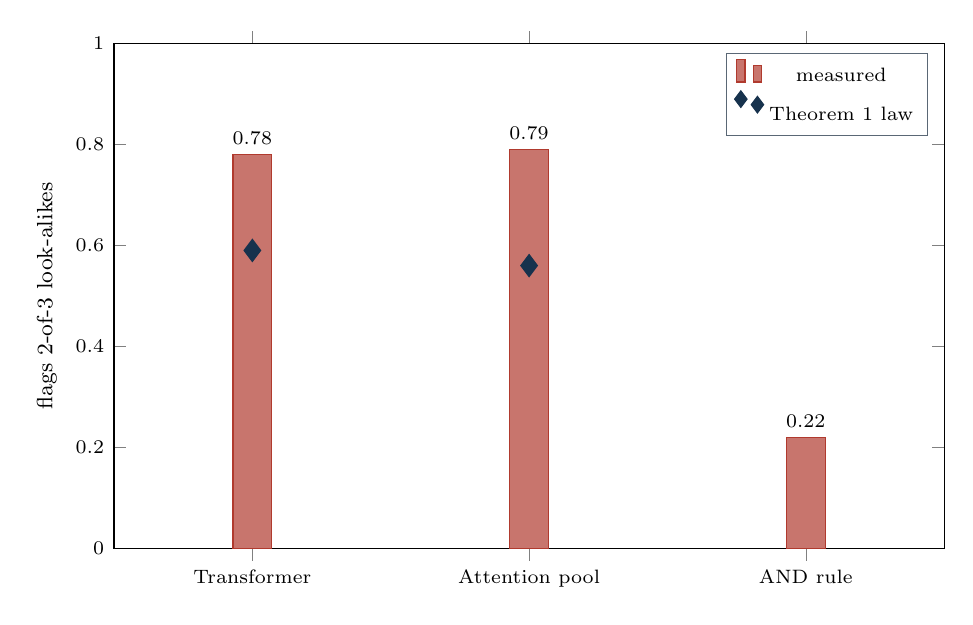
\begin{tikzpicture}
    \begin{axis}[ybar,width=\linewidth,height=0.66\linewidth,ymin=0,ymax=1,bar width=14pt,
      symbolic x coords={Transformer,Attention pool,AND rule},xtick=data,
      ylabel={flags 2-of-3 look-alikes},tick label style={font=\scriptsize},label style={font=\footnotesize},
      enlarge x limits=0.25,nodes near coords,every node near coord/.append style={font=\scriptsize},point meta=explicit symbolic,
      legend style={font=\scriptsize,at={(0.98,0.98)},anchor=north east,draw=Muted}]
      \addplot[fill=Red!70,draw=Red] coordinates {(Transformer,0.78) [0.78] (Attention pool,0.79) [0.79] (AND rule,0.22) [0.22]};
      \addlegendentry{measured}
      \addplot[only marks,mark=diamond*,mark size=4pt,color=Navy,nodes near coords={},forget plot] coordinates {(Transformer,0.59) (Attention pool,0.56)};
      \addlegendimage{only marks,mark=diamond*,mark size=3pt,color=Navy}
      \addlegendentry{Theorem 1 law}
    \end{axis}
  \end{tikzpicture}
  \end{column}
  \begin{column}{0.41\textwidth}
  \vspace{4mm}
  Both models detect Fault 1 well (0.91--0.93) and flag \textbf{most} 2-of-3 look-alikes.
  \vspace{2.5mm}

  They lie about \textbf{0.2 above} the law: the learned attention leans toward an OR, \(\hat\beta=-1.06\). This is Theorem 3 with \(C>k\): 17 of the 20 sensors are not Fault 1's.
  \vspace{2.5mm}

  Fan-coil: \textbf{0.98--0.99} flagged, against 0.33 for the AND rule.
  \end{column}
  \end{columns}
  \vspace{1mm}
  \takeaway{Trained on Normal vs.\ Fault 1, the transformers flag 3 to 4 times more look-alikes than the AND rule.}
  \note{0:45. Result 1, plain training. Bars are the share of two-of-three look-alikes flagged; the diamonds are Theorem 1's law, computed from each model's own detection rate. Both models detect Fault 1 well and flag most look-alikes. They are even about 0.2 above the law, because their attention leans toward an OR: the learned inverse temperature is minus 1.06. That is the third case of Theorem 3, since 17 of the 20 sensors are not Fault 1's. On the fan-coil data they flag 98 to 99 percent, against 33 percent for the AND rule. So without near-misses, the transformers have exactly the false-alarm problem the theory predicts.}
\end{frame}

% Result 2
\begin{frame}[t]{Result 2: near-misses cut false alarms, also on unseen look-alikes}
  \notation{numbers: share of windows flagged by the transformer, plain \(\to\) + near-misses, mean of 3 seeds \(\cdot\) never trained: these look-alikes were not in the training data \(\cdot\) 1\% false alarms on normal windows}
  \vspace{2mm}
  \begin{center}
  {\fontsize{9.6}{12}\selectfont\renewcommand{\arraystretch}{1.4}\setlength{\tabcolsep}{5mm}
  \begin{tabular}{@{}lcc@{}}
    \toprule
    & \textbf{synthetic} & \textbf{fan-coil}\\
    \midrule
    Fault 1 detected & \(0.93\to0.88\) & \(1.00\to1.00\)\\
    2-of-3 look-alikes & \(0.78\to\mathbf{0.15}\) & \(0.99\to\mathbf{0.18}\)\\
    1-of-3 look-alikes {\scriptsize\color{Muted}(never trained)} & \(0.45\to\mathbf{0.03}\) & \(0.96\to\mathbf{0.06}\)\\
    one loud sensor {\scriptsize\color{Muted}(never trained)} & \(1.00\to\mathbf{0.02}\) & \(1.00\to\mathbf{0.05}\)\\
    \midrule
    AND rule on 2-of-3 {\scriptsize\color{Muted}(reference)} & \(0.20\) & \(0.31\)\\
    \bottomrule
  \end{tabular}\par}
  \end{center}
  \vspace{3mm}
  \takeaway{Fault 1 detection barely changes, while false alarms on look-alikes fall to the level of the AND rule or below.}
  \note{0:40. Result 2: the transformer, plain versus with near-misses. Detection of Fault 1 barely changes. Two-of-three look-alikes, the ones we trained on, drop from 0.78 to 0.15 and from 0.99 to 0.18, at or below the AND rule. And look-alikes that were never in training drop too: one sensor and one loud sensor fall to 0.02 to 0.06. That is the generalisation expected from a model that computes an AND.}
\end{frame}

% Result 3
\begin{frame}[t]{Result 3: the learned attention becomes a soft AND}
  \notation{\(\hat\beta\): learned inverse temperature of the attention pool, read from its attention weights \(\cdot\) \(\rho\): share of near-misses in training \(\cdot\) mean of 3 seeds, bars: standard deviation}
  \begin{columns}[c,onlytextwidth]
  \begin{column}{0.66\textwidth}
  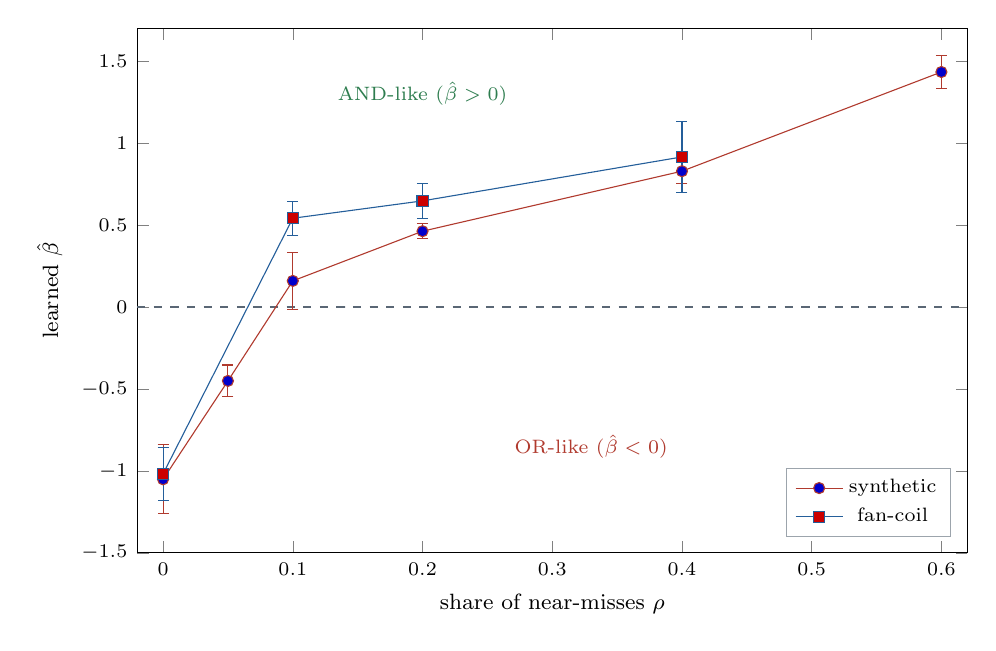
\begin{tikzpicture}
    \begin{axis}[width=\linewidth,height=0.68\linewidth,xmin=-0.02,xmax=0.62,ymin=-1.5,ymax=1.7,
      xlabel={share of near-misses \(\rho\)},ylabel={learned \(\hat\beta\)},
      tick label style={font=\scriptsize},
      legend style={font=\scriptsize,at={(0.98,0.03)},anchor=south east,draw=Muted!60}]
      \addplot[Muted,dashed,domain=-0.02:0.62,forget plot] {0};
      \addplot+[mark=*,color=Red,error bars/.cd,y dir=both,y explicit] coordinates {(0,-1.051) +- (0,0.211) (0.05,-0.451) +- (0,0.097) (0.1,0.159) +- (0,0.175) (0.2,0.462) +- (0,0.047) (0.4,0.828) +- (0,0.073) (0.6,1.433) +- (0,0.099)};
      \addlegendentry{synthetic}
      \addplot+[mark=square*,color=Blue,error bars/.cd,y dir=both,y explicit] coordinates {(0,-1.018) +- (0,0.161) (0.1,0.541) +- (0,0.103) (0.2,0.647) +- (0,0.106) (0.4,0.915) +- (0,0.218)};
      \addlegendentry{fan-coil}
      \node[font=\scriptsize,Green] at (axis cs:0.2,1.3) {AND-like (\(\hat\beta>0\))};
      \node[font=\scriptsize,Red] at (axis cs:0.33,-0.85) {OR-like (\(\hat\beta<0\))};
    \end{axis}
  \end{tikzpicture}
  \end{column}
  \begin{column}{0.31\textwidth}
  {\fontsize{9.4}{11.6}\selectfont The learned \(\hat\beta\) is \textbf{negative} (OR-like) without near-misses, turns \textbf{positive} with them, and grows with their share while staying \textbf{finite}: a soft AND.\par}
  \end{column}
  \end{columns}
  \note{0:30. The plot shows the learned inverse temperature of the attention pool as the share of near-misses grows, on both datasets. Without near-misses it is negative, OR-like, because most sensors are not Fault 1's. With near-misses it turns positive and keeps growing with their share, but it stays finite: a soft AND, as Theorems 3 and 4 predict.}
\end{frame}

% Conclusion and next steps
\begin{frame}[t]{Conclusion and Next Steps}
  \notation{soft AND: finite \(\beta>0\) \(\cdot\) hard AND: \(\beta\to\infty\), the minimum \(\cdot\) head refit: the output weight and bias are fitted at each step}
  \vspace{1mm}
  \begin{thmblock}{Conclusion}
    Training on Normal vs.\ Fault 1 learns the \textbf{SUM}, the optimal rule for the training test, while deployment needs the \textbf{AND}, which no weighted sum can replace.
    Near-misses push softmax attention from the SUM toward the AND, and under noise it settles on a \textbf{soft AND}.
    In transformers, near-misses cut alarms on look-alikes from 0.78--0.99 to 0.02--0.18, including look-alikes never seen in training.
  \end{thmblock}
  \vspace{1.5mm}
  \textbf{Next steps}
  \vspace{0.5mm}
  {\fontsize{8.8}{10.8}\selectfont
  \begin{itemize}\setlength{\itemsep}{1.2mm}
    \item \textbf{Global version.} Done in part: with the head refit, every start with \(\beta(0)\ge0\) ends at an AND (Theorem 3(d)), and a fixed interval around uniform attention reaches the soft AND (Theorem 4(ii)). Next: the full attention layer with learned queries and keys, trained jointly with the head, and starts far on the OR side.
    \item \textbf{Timing.} Near-misses in time, for look-alikes that differ from Fault 1 only in \emph{when} the sensors shift.
    \item \textbf{Field data.} Validation on real data from several units.
  \end{itemize}\par}
  \vspace{1mm}
  {\centering\color{Navy}\bfseries Thank you. Questions?\par}
  \note{0:50. To conclude. Training on normal versus Fault 1 learns the SUM, the optimal rule for the training test, while deployment needs the AND, which no weighted sum can replace. Near-misses push softmax attention toward the AND, and under noise it settles on a soft AND. In transformers they cut false alarms on look-alikes to 2 to 18 percent, including look-alikes never seen in training. Next steps: the global version is done in part, from uniform or AND-leaning starts; what remains is the full attention layer trained jointly with the head, and starts far on the OR side. Then near-misses in time, and field data from several units. Thank you.}
\end{frame}

\end{document}
